% ---------------------------------- AES ---------------------------------------

\documentclass[a4paper,12pt]{book}

%TODO: aggiungere un Abstract? (L'objective (l'obiettivo) di questa ricerca è ...)
%TODO: aggiungere bibliografia.
%TODO: aggiungere indice analitico alla fine del "libro".

%TODO: Aggiungere capitolo: "Implementazione" (implementazione basilare) in C++ e/o Java.

% ----------------------------- BEGIN PREAMBLE ---------------------------------------

\usepackage{lmodern}
\usepackage{alltt, fancyvrb, url}
\usepackage{float}
\usepackage{graphicx}
\usepackage[utf8]{inputenc}
\usepackage{titlesec} %porre titlesec prima di hyperref per evitare il warning "The anchor of a bookmark and its parent's must not(hyperref) be the same".
\usepackage[breaklinks]{hyperref} %porre hyperref infondo al preamble perché altrimenti potrebbe dare warning tipo: "The anchor of a bookmark and its parent's must not(hyperref) be the same" dovuto al fatto che titlesec si trova dopo hyperref.
\usepackage{amsmath,amssymb,amsthm}

\usepackage{geometry} % [showframe] % serve per mostrare il margine, è da rimuovere quando ho finito di controllare il margine. %TODO: remove showframe %TODO: sistemare margini se uso geometry.

\usepackage[italian]{babel}

\usepackage[italian]{cleveref}

\usepackage{comment}
\usepackage[nopatch={eqnum,footnote}]{microtype} %[nopatch={eqnum,footnote}] aggiunto per evitare il warning "patching footnotes failed"
\usepackage{fancyhdr}

\usepackage[scaled=.92]{helvet}
\usepackage[T1]{fontenc}

\usepackage{lscape}

\usepackage{subcaption}

% ------ title -------------------
\usepackage[svgnames]{xcolor}
\ifpdf
\usepackage{pdfcolmk}
\fi
%% check if using xelatex rather than pdflatex
\ifxetex
\usepackage{fontspec}
\fi
%% drawing package
\usepackage{tikz}
%% for dingbats
\usepackage{pifont}
\providecommand{\HUGE}{\Huge}% if not using memoir
\newlength{\drop}
% ------ end title -------------------

% ------ chapter style -----------
\usepackage{kpfonts}
\usepackage{xcolor,calc, blindtext}
\definecolor{chaptercolor}{gray}{0.8}
% ------ end chapter style -----------

% ----- font family ------------------

%\usepackage{tgbonum}
%\fontfamily{cmss}\selectfont

\fontencoding{T1}
\fontfamily{garamond}
\fontseries{m}
%\fontshape{it}
%\fontsize{12}{15}
\selectfont %da warning forse perché viene usato \bfseries\scshape

%\usepackage{utopia} %utopia è obsoleto; usare fourier al posto.
% ----- end font family ------------------

% ------ section ---------

% ------ end section ---------

\usepackage{longtable}

% ---- ornamenti (distaccamenti) ---------

% per gli ornamenti, servono per distaccare parti del testo.
\usepackage{fourier-orns}

\newcommand{\fleuron}{
	\par\nopagebreak
	\parbox{\linewidth}{
		\centering\bigskip\aldineleft\par\bigskip
	}
}

\newcommand{\ornament}{
	\par\nopagebreak
	\parbox{\linewidth}{
		\centering\bigskip$\ast$\par$\ast\quad\ast$\par\bigskip
	}
}

% ---- ornamenti (distaccamenti) end ---------

% ----- firma (signature) begin ----------------

%\usepackage{emerald} %questo non lo trova
\usepackage{frcursive}
\usepackage{inslrmin}

\usepackage{soul} % per la sottolineatura.
\usepackage{setspace} % prima aveva anche l'option [doublespacing], ma dava errore.

% ----- firma (signature) end ----------------

% ----- per molteplici colonne begin ----------------

\usepackage{multicol}

% ----- per molteplici colonne end ----------------

% ----- empty page command begin -------------

\newcommand\blankpage{% comando pagina vuota
	\clearpage
	\begingroup
	\null
	\thispagestyle{empty}%
	\addtocounter{page}{-1}%
	\hypersetup{pageanchor=false}%
	\clearpage
	\endgroup
}

% ----- empty page command end -------------

% ----- code ----------------
%TODO: remove

\usepackage{listingsutf8}

\definecolor{codegreen}{rgb}{0,0.6,0}
\definecolor{codegray}{rgb}{0.5,0.5,0.5}
\definecolor{codepurple}{rgb}{0.58,0,0.82}
\definecolor{backcolour}{rgb}{0.95,0.95,0.92}
\definecolor{myblue}{rgb}{0.3, 0.6, 0.8}
\definecolor{myblue2}{rgb}{0.11, 0.19, 0.46}
\definecolor{myblue3}{rgb}{0.27, 0.55, 0.81}

% VS2017 C++ color scheme
\definecolor{clr-background}{RGB}{255,255,255}
\definecolor{clr-text}{RGB}{0,0,0}
\definecolor{clr-string}{RGB}{163,21,21}
\definecolor{clr-namespace}{RGB}{0,0,0}
\definecolor{clr-preprocessor}{RGB}{128,128,128}
\definecolor{clr-keyword}{RGB}{0,0,255}
\definecolor{clr-type}{RGB}{43,145,175}
\definecolor{clr-variable}{RGB}{0,0,0}
\definecolor{clr-constant}{RGB}{111,0,138} % macro color
\definecolor{clr-comment}{RGB}{0,128,0}

\definecolor{weborange}{RGB}{255,165,0}

\lstdefinestyle{VS2017}{
	backgroundcolor=\color{clr-background}, % oppure darkgray o darkgrey %TODO: mettere quello classico.
	basicstyle=\color{clr-text}, % any text
	stringstyle=\color{clr-string},
	identifierstyle=\color{clr-variable}, % just about anything that isn't a directive, comment, string or known type
	commentstyle=\color{clr-comment},
	directivestyle=\color{clr-preprocessor}, % preprocessor commands
	% listings doesn't differentiate between types and keywords (e.g. int vs return)
	% use the user types color
	keywordstyle=\color{clr-type},
	keywordstyle={[2]\color{clr-constant}}, % you'll need to define these or use a custom language
	breaklines=true,
	showspaces=false,
	showstringspaces=false,
	%otherkeywords={>,<,.,;,-,!,=,~},
	morekeywords={\#, std, std::cout, cout, std::endl, endl, ::, ifndef, define, endif, pragma, override, decltype, noexcept, alignas, alignof, constexpr, assert, nullptr}, % \# non funziona.
	%keywordstyle=\color{weborange},
	tabsize=4
}

\lstdefinestyle{mystyle}{
	backgroundcolor=\color{backcolour},   
	commentstyle=\color{codegreen},
	keywordstyle=\color{myblue2}, % prima era magenta
	numberstyle=\tiny\color{codegray},
	stringstyle=\color{codepurple},
	basicstyle=\ttfamily\footnotesize,
	breakatwhitespace=false,         
	breaklines=true,                 
	captionpos=b,                    
	keepspaces=true,                 
	numbers=left,                    
	numbersep=5pt,                  
	showspaces=false,                
	showstringspaces=false,
	showtabs=false,                  
	tabsize=2
	%classoffset=1, % starting new class
	%otherkeywords={>,<,.,;,-,!,=,~},
	%morekeywords={>,<,.,;,-,!,=,~},
	%keywordstyle=\color{red},
	%classoffset=0,
}

%\lstset{inputencoding=utf8/latin1} % Questo non andava.

\lstset{language=C++,texcl=true} % questo mi ha fixato il problema delle lettere
% accentate nei commenti, ma non nelle stringhe " " del codice.

% Altrimenti sempre per il problema delle lettere accentat, si può usare questo:
% Anzi questo mi aiuta per le stringhe nel codice " ".
%\begin{comment}
\lstset{
	literate=%
	{á}{{\'a}}1
	{à}{{\`a}}1
	{ã}{{\~a}}1
	{é}{{\'e}}1
	{è}{{\`e}}1
	{ê}{{\^e}}1
	{í}{{\'i}}1
	{ó}{{\'o}}1
	{õ}{{\~o}}1
	{ú}{{\'u}}1
	{ü}{{\"u}}1
	{ù}{{\`u}}1
	{ç}{{\c{c}}}1
	{¡}{{\'!}}1
}
%\end{comment}

\lstset{style=VS2017}

%frame (ovvero un box) attorno al codice
\begin{comment}
	\usepackage[most]{tcolorbox}
	\usepackage{inconsolata}
	
	\newtcblisting[auto counter]{listingframe}[2][]{sharp corners, 
		fonttitle=\bfseries, colframe=gray, listing only, 
		listing options={basicstyle=\ttfamily,language=java}, 
		title=Listing \thetcbcounter: #2, #1}
\end{comment}

% ------ end code -----------

% hyperref settings
\hypersetup{
	colorlinks=true,
	linkcolor=black, %blue
	filecolor=magenta,      
	urlcolor=cyan,
	pdftitle={Sharelatex Example},
	bookmarks=true, %commentato per via del warning
	pdfpagemode=FullScreen,
}

% ----------------------------- END PREAMBLE -----------------------------------------

% ----------------------------- BEGIN CHAPTER STYLE ----------------------------------

% ================== Chapter Style 1 ================================================

%\definecolor{gray75}{gray}{0.75}
%\newcommand{\hsp}{\hspace{20pt}}

%\titleformat{\chapter}[hang]{\Huge\bfseries}{\thechapter\hsp\textcolor{gray75}{|}\hsp}{0pt}{\Huge\bfseries}

% ================== Chapter Style 2 ================================================

%Options: Sonny, Lenny, Glenn, Conny, Rejne, Bjarne, Bjornstrup
\usepackage[Lenny]{fncychap}

% ----------------------------- END CHAPTER STYLE ------------------------------------


% ----------------------------- BEGIN SECTION STYLE ----------------------------------

\titleformat
{\section} % command
[display] % shape
{\bfseries\Large\itshape} % format
{} % label
{0.5ex} % sep
{
	\vspace{1ex} % prima era 1ex
	\rule{\textwidth}{2pt} % 2pt
	\centering
} % before-code
[
\vspace{-2ex}% 2ex
\rule{\textwidth}{1.5pt} % prima era 1.5 col font classico.
] % after-code

% ----------------------------- END SECTION STYLE ------------------------------------

% ----------------------------- BEGIN SUBSECTION STYLE -------------------------------

\titleformat{\subsection}{\centering\bfseries\Large\itshape}{}{}{}

% ----------------------------- END SUBSECTION STYLE ---------------------------------

% ----------------------------- BEGIN SUBSUBSECTION STYLE ----------------------------

\titleformat{\subsubsection}{\centering\bfseries\large\itshape}{}{}{}

% ----------------------------- END SUBSUBSECTION STYLE ------------------------------

% ----------------------------- BEGIN PARAGRAPH STYLE --------------------------------

\titleformat{\paragraph}{\centering\bfseries\normalsize}{}{}{}

% ----------------------------- END PARAGRAPH STYLE ----------------------------------

% ----------------------------- BEGIN TABLE OF CONTENTS ------------------------------

\setcounter{tocdepth}{4}
\setcounter{secnumdepth}{1}

% ----------------------------- END TABLE OF CONTENTS --------------------------------

%\usepackage{enumitem}
%\setlist[description]{style=nextline}
%\leavevmode

\newcommand*{\titleRF}{\begingroup% Robert Frost, T&H p 149
	%\FSfont{5bp} % FontSite Bergamo (Bembo)
	%49
	\drop = 0.2\textheight
	\centering %TODO: questo centering da problemi; uncomment
	\vfill
	{\Huge Advanced Encryption Standard}\\[\baselineskip]
	{\Huge AES}\\[\baselineskip]
	{\large Luca Rengo}\\[0.5\drop]
	{\Large }%\\[0.5\baselineskip] %TODO: \plogo da problemi; questo \\ dava l'errore: "there is no line to end here"
	{\Large The Publisher}\par %TODO: al posto di The Publisher scrivere qualcos'altro
	{\large \scshape year 2022} 
	\vfill\null
	\endgroup}

% ----------------------------- END TITLE PAGE ---------------------------------------

% ----------------------------- BEGIN DOCUMENT ---------------------------------------

\begin{document}
	
	\frontmatter
	
	\titleRF
	
	\tableofcontents
	
	% \input: import the commands from filename.tex to target file.
	
	% \include: does a \clearpage and does an \input.
	
	% \import: needs \usepackage{import} and it's used only when the imported files needs the path. \import{path}{filename}
	
	\mainmatter
	
	%TODO: magari non serve l'introduzione per ogni capitolo? %TODO: remove
	
	%TODO: Abstracts
	
	% ================================ STORIA DI AES ======================================

\chapter{Storia di AES}

% ======================================================================================


% ---------------------------- SECTION: INTRODUZIONE ----------------------------------

%\newpage

\section{Introduzione}

%TODO: \textsf o \textsc o altro ?

%TODO: a blocchi simmetrico o a blocchi simmetrici?
\textsf{\small \textbf{AES} (\emph{\textbf{A}dvanced \textbf{E}ncryption \textbf{S}tandard}) è un cifrario a blocchi simmetrico, inventato da due matematici belghi, Vincent Rijmen e Joan Daemen, da cui viene il nome \emph{Rijndael}, nel 1998 per sostituire il precedente standard: DES (\emph{\textbf{D}ata \textbf{E}ncryption \textbf{S}tandard}).}

%TODO: aggiungere la differenza tra AES e Rijndael, sono diversi.
%TODO: Rijndael: gestisce blocchi e chiavi di differenti dimensioni. (blocco e chiave di 32 bit con 128 bit come minimo e 256 come massimo).
%TODO: AES: gestisce un blocco di dimensione fissa (128 bit) e la chiave può essere da 128, 192 o 256.

% ---------------------------- SECTION: STORIA DI AES ---------------------------------

%\newpage %TODO: questo newpage da problema, è da fixare

\section{Breve storia di AES} 

%TODO: Partire dal DES, dai problemi del DES e del triplo DES
%TODO: Nist 1997
%TODO: I concorrenti di AES: serpent, twofish, ecc. e dire per quale motivo è stato scelto Rijndael come AES alla fine.

\textsf{\small DES era divenuto lo standard dopo un bando dell'NBS (\emph{\textbf{N}ational \textbf{B}ureau of \textbf{S}tandards}), oggi NIST \emph{(\textbf{N}ational \textbf{I}nstitute for \textbf{S}ecurity and \textbf{T}echnology)} per trovare un buon e sicuro algoritmo per proteggere le comunicazioni private dei cittadini americani.}

%TODO: "rettificandone" o "alterandone"
\textsf{\small Venne così proposto un algoritmo chiamato \emph{Lucifer}, sviluppato dall'\emph{IBM} che dopo esser stato modificato dall'NSA (\emph{\textbf{N}ational \textbf{S}ecurity \textbf{A}gency}), riducendone la grandezza della chiave da 128 a 56 bits e rettificandone le funzioni contenute nell'S-box, venne designato come \emph{Data Encryption Standard} (\textbf{DES}).}

%TODO: "in lungo e in largo" magari è poco raffinata come espressione.
%TODO: questa è da rivedere! Mi sembra abbia poco senso compiuto
\textsf{\small DES regnò per 20 anni, venne studiato in lungo e in largo dagli accademici e criptoanalisi di tutto il mondo, grazie a ciò, ci fu finalmente per la prima volta un cifrario certificato che tutti potevano studiare: nacque così il moderno campo della crittografia.}

\textsf{\small Negli anni, molti sfidarono DES e dopo diverse battaglie fu finalmente sconfitto.} %TODO: ampliare come venne sconfitto?

%TODO: "fermare" o "ovviare"
%TODO: magari spiegare perché era lento più nel dettaglio. (perché combinevamo il des tre volte)
\textsf{\small L'unico modo per ovviare a questi attacchi era quello di combinare des tre volte, formando il 3DES (\emph{Triplo DES}). Il problema di questo però era la sua lentezza.} %TODO: estremamente lento


%TODO: "indire" è il verbo corretto?
\textsf{\small Per questo, nel 1997, il NIST indisse un nuovo bando per cercare un nuovo algoritmo di cifratura, forte come il triplo-DES, ma veloce e flessibile.}

\begin{figure}[H]
	\centering
	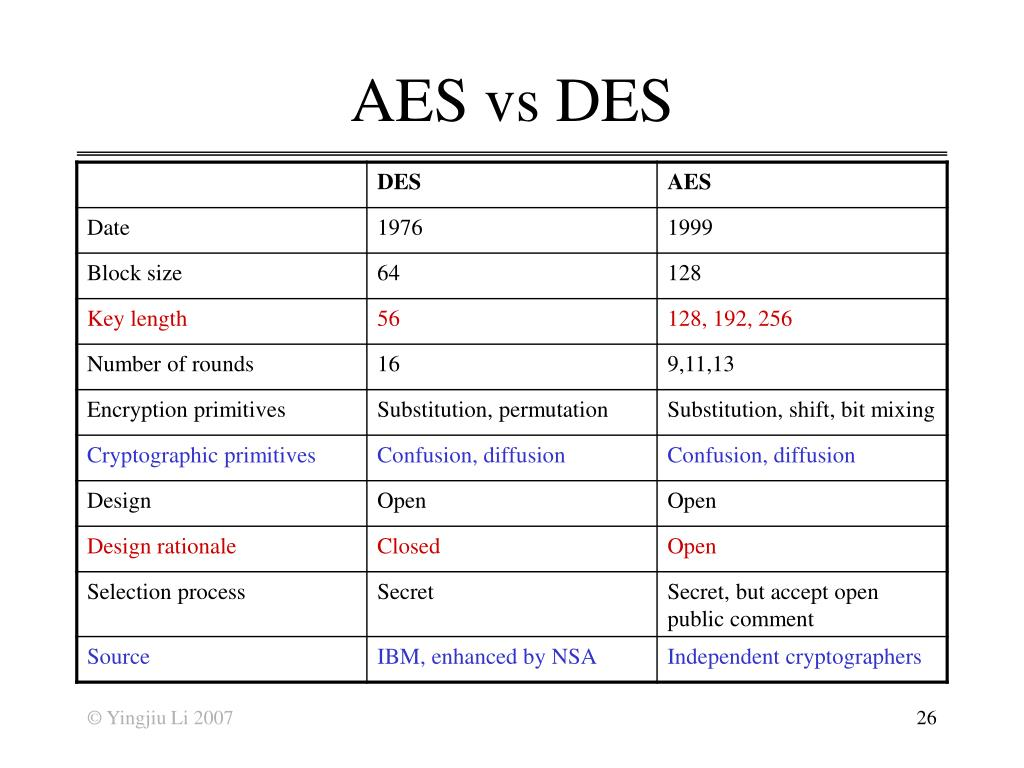
\includegraphics[width=1\textwidth, height=1\textheight, keepaspectratio]{./images/des_vs_aes/aes-vs-des.png}
	\caption{AES vs DES}
	\label{fig:aes_vs_des}
\end{figure}

%TODO: "spuntò" o "emerse" ?
%TODO: "semplicità"? Approfondire un po' di più magari
\textsf{\small Vari algoritmi compitero: Serpent, Twofish, MARS, RC6, ma alla fine spuntò Rijndael per la sua semplicità e velocità.}

% ---------------------------- SECTION: AES VS RIJNDEAL ------------------------------

%\newpage

\section{AES vs Rijndeal}

\textsf{\small AES è un'implentazione di Rijndael, divenuto l'algoritmo di cifratura standard del governo degli Stati Uniti d'America.}
\textsf{\small Una differenza tra i due è che AES utilizza blocchi di dati da 128 bits, mentre Rijndael permette oltre a blocchi da 128, anche blocchi da 192 e 256 bits.} %TODO: "blocchi di dati"?

\textsf{\small Sia AES che Rijndael permettono una grandezza della chiave di 128, 192 o 256 bits, da cui ne ricaviamo il numero di rounds: 10, 12 o 14 rispettivamente.}

\begin{comment}
\begin{figure}[H]
	\centering
	\includegraphics[width=1\textwidth, height=1\textheight, keepaspectratio]{./images/.png}
	\caption{}
	\label{fig: }
\end{figure}
\end{comment}

%TODO: immagine AES vs Rijndael

% ------------------------ SECTION: SYMMETRIC VS ASYMMETRIC? --------------------------

%\newpage

\section{Cifratura simmetrica vs asimmetrica} %rinominare in "Cifrari simmetrici vs asimettrici"?

\textsf{\small Nella cifratura simmetrica viene usata una chiave sia per la cifratura che per la decifratura di un messaggio.}

\textsf{\small La cifratura asimmetrica è basata sul concetto di chiave pubblica e chiave privata. Vengono, quindi usate due chiavi sia per la cifratura che per la decifratura. Usiamo la chiave pubblica per cifrare il messagio e la chiave privata per decifrarlo.} %TODO: qui sto facendo un po' di controsenso.

\textsf{\small Ulteriori differenze: }

\begin{tabular}{|c|c|}
	\hline
	\textbf{Simmetrico} & \textbf{Asimmetrico} \\
	\hline
	\textsf{\small Richiede una sola  } & \textsf{\small Richiede due chiavi, } \\
	\textsf{\small chiave sia} & \textsf{\small  una pubblica e una privata,} \\
	\textsf{\small per la cifratura } & \textsf{\small una per cifrare e } \\
	\textsf{\small che la decifratura.} & \textsf{\small una per decifrare.} \\
	\hline
	\textsf{\small Lo spazio del testo cifrato è  } & \textsf{\small Lo spazio del testo cifrato è  } \\
	\textsf{\small lo stesso o più piccolo } & \textsf{\small lo stesso o più grande } \\
	\textsf{\small del messaggio originale.} & \textsf{\small del messaggio originale.} \\
	\hline
	\textsf{\small Il processo di cifratura } & \textsf{\small Il processo di cifratura } \\
	\textsf{\small è molto veloce.} & \textsf{\small è molto lento.} \\
	\hline
	\textsf{\small È usato quando un  } & \textsf{\small È usato per trasferire } \\
	\textsf{\small grosso ammontare di dati} & \textsf{\small piccole quantità} \\
	\textsf{\small deve essere trasferito.} & \textsf{\small  di dati.} \\
	\hline
	\textsf{\small Fornisce solamente } & \textsf{\small Fornisce confidenzialità, } \\ %TODO: non ripudio
	\textsf{\small la confidenzialità.} & \textsf{\small autenticità e non ripudio.} \\
	\hline
	\textsf{\small La chiave usata è di solito } & \textsf{\small La lunghezza della chiave } \\
	\textsf{\small di lunghezza 128 o 256 bits.} & \textsf{\small è di 2048 o più bits.} \\
	\hline
	\textsf{\small L'utilizzo delle risorse è basso.} & \textsf{\small L'utilizzo di risorse è alto.} \\
	\hline
	\textsf{\small Esempi: DES, 3DES, } & \textsf{\small Esempi: DSA, RSA, } \\
	\textsf{\small AES, RC4} & \textsf{\small Diffie-Hellman, ECC, El Gamal} \\
	%\textsf{\small } & \textsf{\small } \\
	\hline
\end{tabular}

\begin{figure}[H]
	\centering
	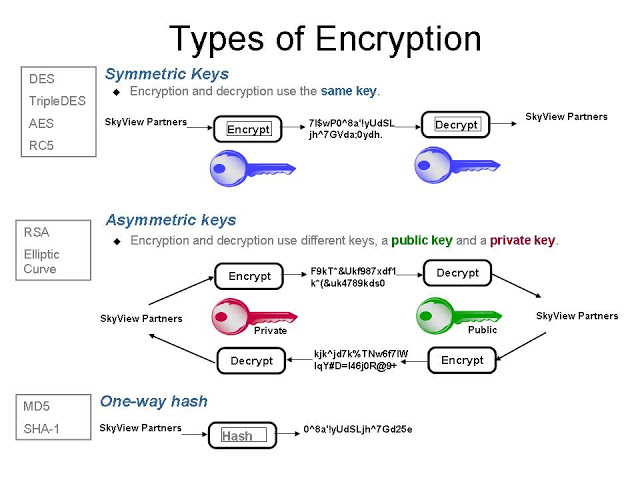
\includegraphics[width=1\textwidth, height=1\textheight, keepaspectratio]{./images/types_of_encryptions/types_of_encryption.png}
	\caption{Tipi di cifratura}
	\label{fig:encryption_types}
\end{figure}

\textsf{\small AES è di tipo simmetrico, quindi useremo la stessa chiave sia per criptare il nostro messaggio sia per decriptarlo. }

\begin{figure}[H]
	\centering
	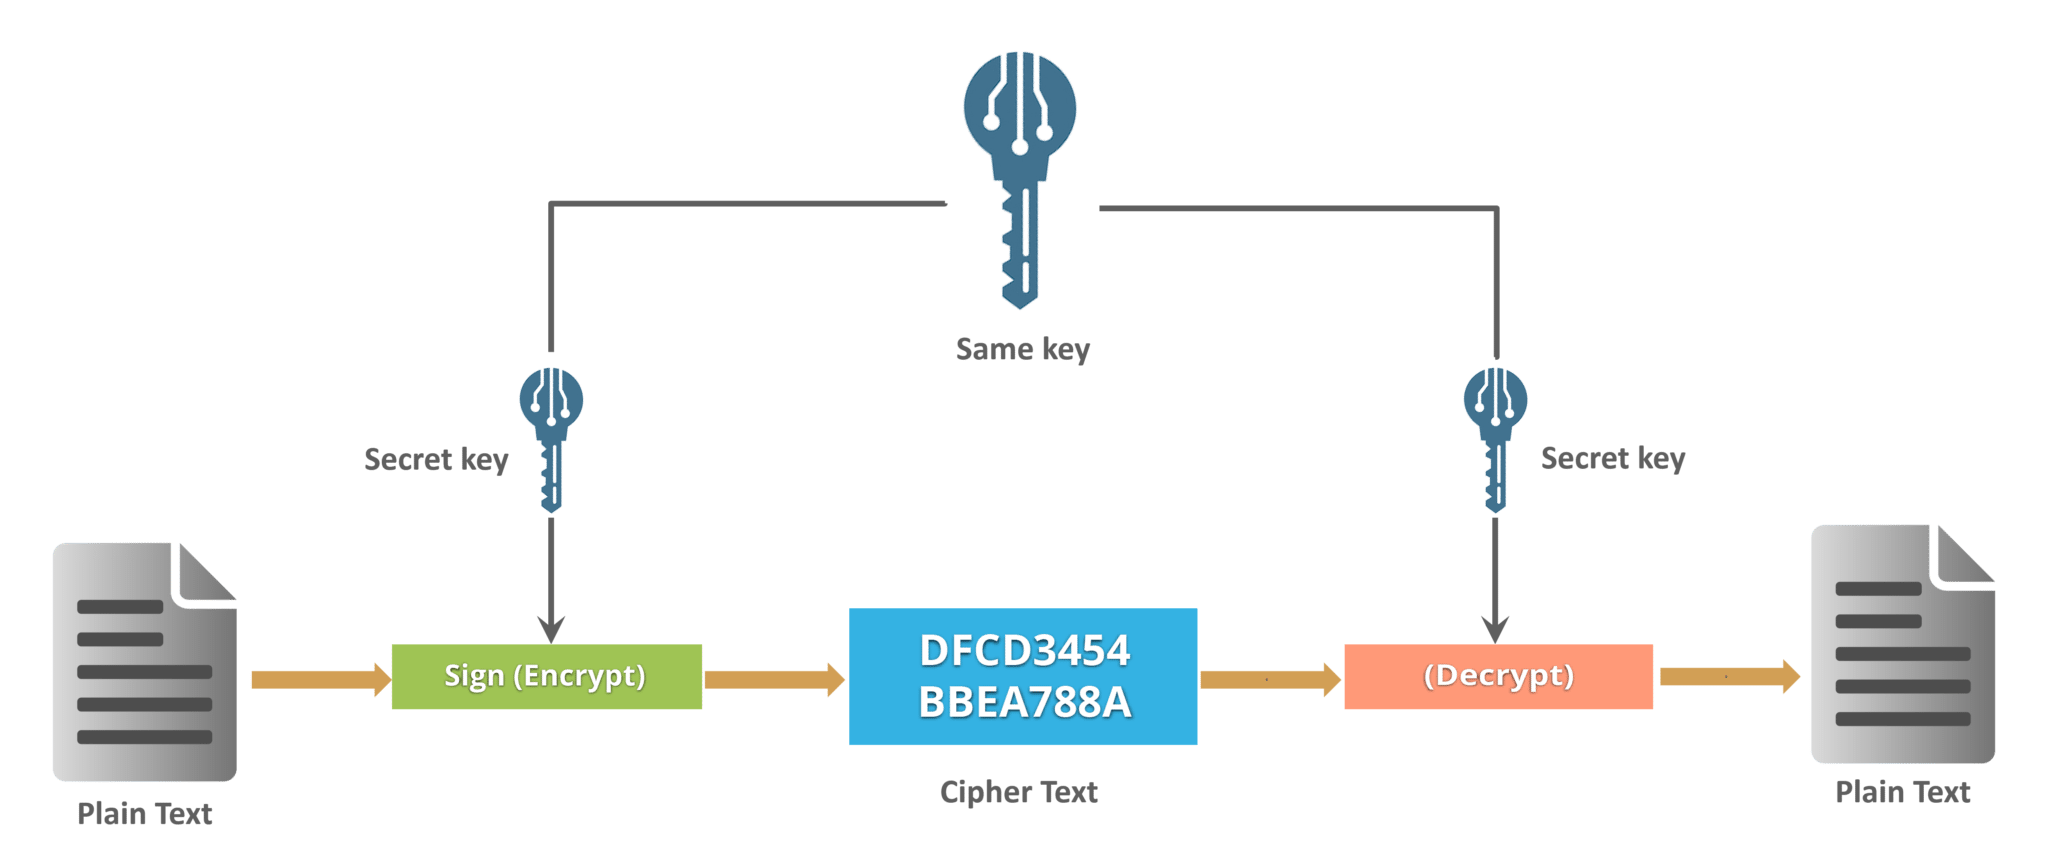
\includegraphics[width=1\textwidth, height=1\textheight, keepaspectratio]{./images/types_of_encryptions/symmetric_vs_asymmetric/symmetric-key-what-is-cryptography.png}
	\caption{Cifratura a chiave simmetrica}
	\label{fig:symmetric_encryption}
\end{figure}

% -------------------------------- FINE CAPITOLO --------------------------------------
	
	% ================================ L'ALGORITMO ========================================

\chapter{L'Algoritmo} %TODO: Rinominare in "Una panoramica sull'Algoritmo" o in realtà quello è per una sezione?

%TODO: Le varie sezioni: sub bytes, Shift Rows, mix columns, Add Round Key
%TODO: aggiungere immagini

%TODO: perché l'ultimo round è differente?

%TODO: 1. KeyExpansion (Rijndael Key Scheduler/AES Key Scheduler)
%TODO: 1. AddRoundKey (con lo XOR)

%TODO: 1. SubBytes (S-Box)
%TODO: 2. ShiftRows (1a riga niente, 2a riga = shift a sinistra di 1, 3a riga = shift di 2, 4a riga = shift di 3) (lo shift è come una ROL in x86)
%TODO: 3. MixColumns (Rijndael Key Scheduler/AES Key Scheduler)
%TODO: 4. AddRoundKey (con lo XOR)

%TODO: ShiftRows e MixColumns per la "Confusione e Diffusione" (teoria di Shannon).

%TODO: 10 rounds (fasi/cicli) per chiavi di 128-bit
%TODO: 12 rounds (fasi/cicli) per chiavi di 192-bit
%TODO: 14 rounds (fasi/cicli) per chiavi di 256-bit

% ======================================================================================

% ---------------------------- SECTION: INTRODUZIONE ----------------------------------

%\newpage

\section{Introduzione}

\index{AES}

\textsf{\small In questo capitolo, tratteremo il funzionamento dell'algoritmo di AES con una panoramica dall'alto, per poi affrontare nel prossimo capitolo, più in dettaglio, la sua matematica.}

% ----------------- SECTION: I TRE CONCETTI DIETRO LA CRITTOGRAFI ----------------------

%\newpage

\section{I tre concetti dietro la Crittografia} %TODO: Le tre idee/concetti/principi dietro la/alla Crittografia

\index{Shannon} \index{diffusione} \index{confusione} \index{teoria dell'informazione} \index{simmetrica}

\textsf{\small Alla base della crittografia, ci sono due importanti proprietà dei cifrari a chiave simmetrica, elaborati dal padre della teoria dell'informazione, Claude Elwood Shannon, ovvero: \emph{diffusione} e \emph{confusione}.} \\

\begin{comment}
\begin{figure}[H]
	\centering
	\includegraphics[width=1\textwidth, height=1\textheight, keepaspectratio]{./images/theory_of_information/confusion_and_diffusion.png}
	\caption{Confusion and Diffusion}
	\label{fig:confusion_and_diffusion2}
\end{figure}
\end{comment}

%TODO: itemize?

\textsf{\small Il principio della \emph{confusione} vela la connessione tra il messaggio originale e il testo cifrato.} %TODO: messaggio/testo; [per esempio cifrario di cesare (con annessa immagine volendo)]

\textsf{\small La proprietà di \emph{diffusione}, invece, riguarda lo scombussolamento della posizione dei caratteri del messaggio.} %TODO: [un semplice esempio potrebbe essere la trasposizione delle colonne in una matrice oppure non lo scrivo.]

\index{segretezza della chiave}

\textsf{\small Un altro importante concetto è quello della \emph{segretezza della chiave}, ovvero che l'algoritmo alla base del cifrario è conosciuto, è pubblico, ma la sola conoscenza di questo non è sufficiente per poter conseguire l'accesso alle informazioni, perché per poter attingerle sarà necessario conoscere la chiave segreta.} %TODO: nella/della chiave; attingere/ottenere; attingerle/acquisire/raggiungere; concetto/astrazione

\begin{figure}[H]
	\centering
	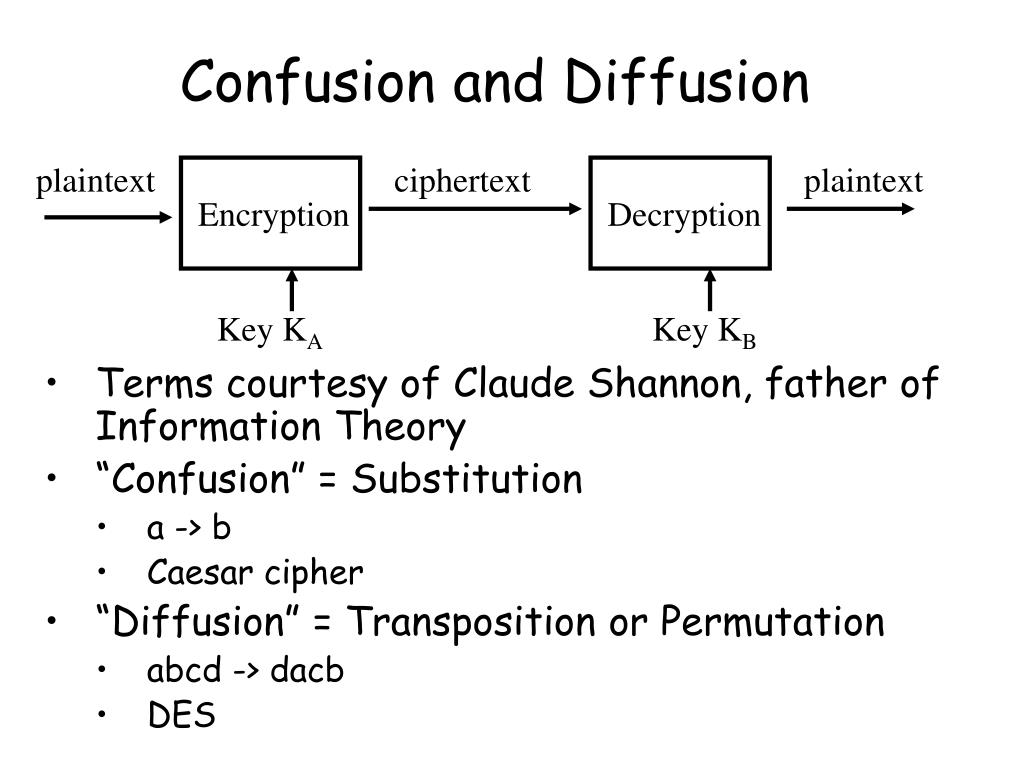
\includegraphics[width=1\textwidth, height=1\textheight, keepaspectratio]{./images/theory_of_information/confusion-and-diffusion.png}
	\caption{Confusione e Diffusione}
	\label{fig:confusion_and_diffusion}
\end{figure}

%TODO: [volendo aggiungere altro sulla teoria dell'informazione, su Shannon, sull'importanza, ecc. Magari aggiungere anche un'immagine.]

%TODO: [aggiungere una o più immagini sulla teoria di Shannon]

% ------------------- SECTION: UNA PANORAMICA SULL'ALGORITMO --------------------------

\section{Una panoramica sull'Algoritmo} %TODO: Una panoramica dell'Algoritmo/Una panoramica sull'Algoritmo (meglio una panoramica sull'algoritmo come nome!) oppure "L'Algoritmo in breve" o "Semplice Overview dell'Algoritmo".

%TODO: itemize?
%TODO: forse dovrei semplificarlo un attimo e parlarne più con calma prima di passare alle liste delle operazioni.

\index{state matrix} \index{matrice di stato} \index{sub-bytes} \index{mix columns} \index{shift rows} \index{add round key}

\textsf{\small I dati di input vengono caricati in una matrice 4x4, anche chiamata \emph{state matrix} (matrice di stato), dove ogni cella rappresenta 1 byte di informazione e su queste compiamo diverse operazioni: \emph{sub bytes} (sostituzione dei bytes), \emph{shift rows} (spostamento delle righe), \emph{mix columns} (mescolamento delle colonne), \emph{add round key} (aggiunta della chiave del round) per un numero di volte, di rounds pari alla grandezza della chiave.} %TODO: oppure metterli in un itemize?

\begin{figure}[H]
	\centering
	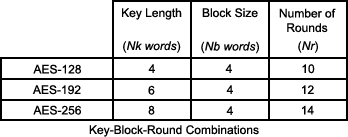
\includegraphics[width=0.8\textwidth, height=0.8\textheight, keepaspectratio]{./images/aes/key_size_and_number_of_rounds.png}
	\caption{Key Size e Numero di Rounds}
	\label{fig:aes_key_size_number_of_rounds}
\end{figure}

\index{XOR}

\textsf{\small Nel primo round svolgiamo uno XOR tra il messaggio d'input e la chiave segreta.}

\textsf{\small Lo \emph{XOR} (\emph{E\textbf{X}clusive-\textbf{OR}}) bit-a-bit è un'operazione di macsheratura dei bit, dove se i due bit di input sono diversi, allora produrrà un 1 in uscita, altrimenti se sono uguali, uno zero.} 

\begin{figure}[H]
	\centering
	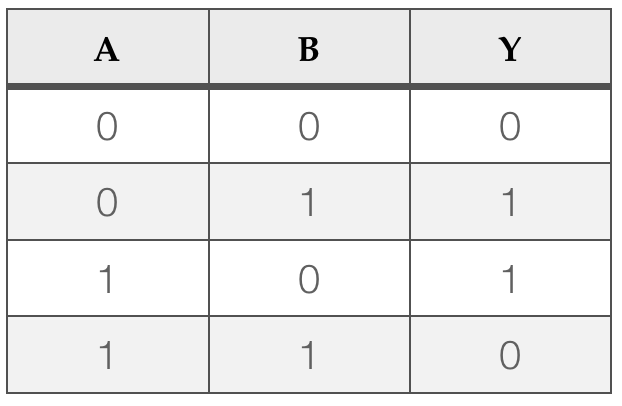
\includegraphics[width=0.6\textwidth, height=0.6\textheight, keepaspectratio]{./images/XOR/XOR-Truth-Table.png}
	\caption{Tabella della verità dello XOR}
	\label{fig:xor_truth_table}
\end{figure}

\subsection{Perché lo XOR è usato in crittografia?}

\index{XOR} \index{AND} \index{OR} \index{NOT}

\begin{itemize}
	\item \textsf{\small Lo XOR non \emph{leaka} informazioni sull'input originale.} %TODO: magari leaka non è proprio il top come parola, non esiste nemmeno in italiano
	\item \textsf{\small Lo XOR è una \emph{involutory function} (funzione involutoria) tale che se la applichi due volte riottieni il testo originale.}
	\item \textsf{\small L'output dello XOR dipende da entrambi gli input. Non è così per le altre operazioni (AND, OR, NOT, ecc.).}
\end{itemize}

\fleuron

%TODO: magari semplificare questa parte.

\subsection{Key Expansion | Key Schedule} %TODO: remove?

\index{key expansion} \index{key schedule} \index{rounds} \index{chiavi}

\textsf{\small Per poter elaborare i rounds, l'algoritmo ha bisogno di molte chiavi, una per round, queste vengono tutte derivate dalla chiave iniziale.}

%TODO: Fare una subsection?: titolo: "Come vengono ottenute le chiavi per ogni round?" oppure no? KEY EXPANSION/KEY SCHEDULE
%TODO: Per poter eseguire/elaborare i rounds, l'algoritmo ha bisogno di molte chiavi [una per round?], queste vengono tutte derivate dalla chiave iniziale. (volendo scrivere: Questo è uno dei motivi per cui AES viene criticato, perché tutte le chiavi vengono derivate dalla chiave originale).

\textsf{\small Il procedimento per ricavarle è questo: }

\index{XOR} \index{round constant}

\begin{enumerate}
	\item \textsf{\small Sposta la prima cella dell'ultima colonna della precedente chiave in fondo alla colonna.} %TODO: spostare
	\item \textsf{\small Ogni byte viene posto in una substitution box che lo mapperà in qualcos'altro.} %TODO: (S-box) dopo substitution box; specificare cosa quel qualcos'altro.
	\item \textsf{\small Viene effettuato uno XOR tra la colonna e una \emph{round constant} (costante di round) che è diversa per ogni round.} %TODO: approfondire come è diversa.
	\item \textsf{\small Infine viene realizzato uno XOR con la prima colonna della precedente chiave.}
	%\item \textsf{\small }
\end{enumerate}

\index{XOR}

\textsf{\small Per le altre colonne, vengono semplicemente eseguiti degli XOR con la stessa colonna della precedente chiave (eccetto per le chiavi a 256 bit che hanno un procedimento un po' più complicato).} %TODO: rimuovere la parte tra parentesi? ovvero la parte procedimento un po' più complicato o approfondirla?

\begin{figure}[H]
	\centering
	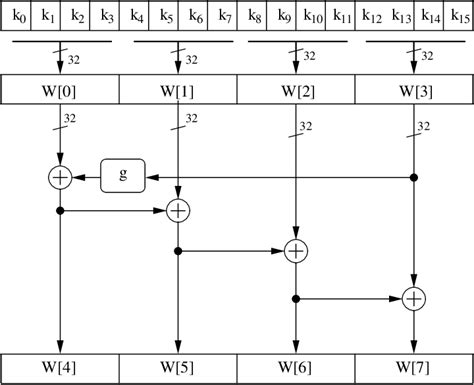
\includegraphics[width=0.8\textwidth, height=0.8\textheight, keepaspectratio]{./images/key_expansion/key_expansion.png}
	\caption{Key Expansion}
	\label{fig:key_expansion}
\end{figure}

\index{AES}

\textsf{\small La singola chiave viene espansa in 11 chiavi per AES-128, 13 per AES-192 e 15 per AES-256.}

\index{RotWord} \index{SubWord} \index{Rcon} \index{XOR}

\textsf{\small Ogni byte della chiave viene inserita in vari arrays, in cui verranno eseguite delle specifiche operazioni: \emph{RotWord}, \emph{SubWord}, \emph{Rcon} e infine verranno eseguiti degli XOR tra loro.}

\begin{figure}[H]
	\centering
	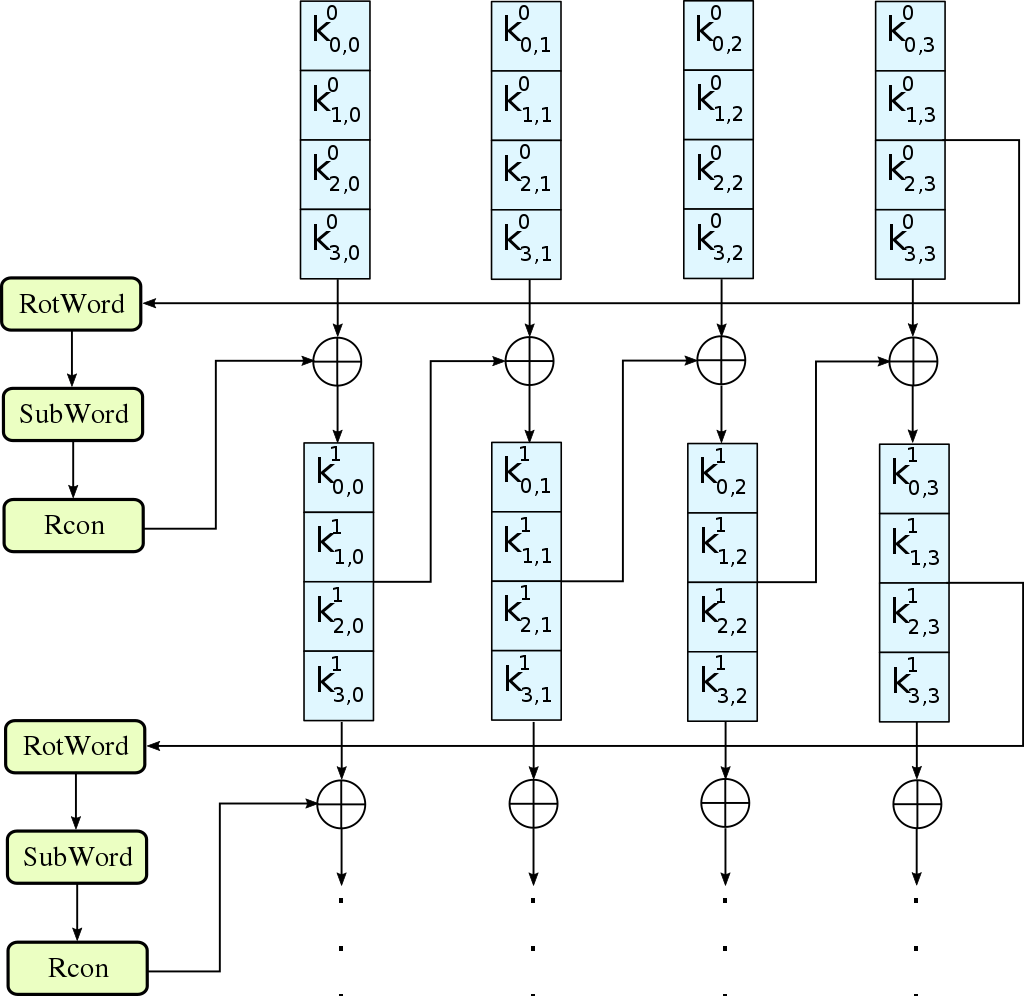
\includegraphics[width=0.6\textwidth, height=0.6\textheight, keepaspectratio]{./images/key_expansion/AES-Key_Schedule_128-bit_key.png}
	\caption{Key Expansion}
	\label{fig:key_expansion2}
\end{figure}

\subsubsection{RotWord}

\index{RotWord}

\textsf{\small Questa funzione ruota una word di 32 bits.}

\begin{figure}[H]
	\centering
	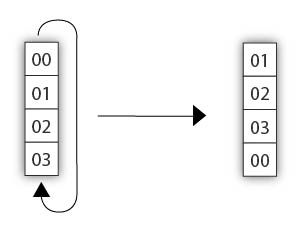
\includegraphics[width=0.4\textwidth, height=0.4\textheight, keepaspectratio]{./images/key_expansion/key_schedule-rot_word.png}
	\caption{Rot Word}
	\label{fig:rot_word2}
\end{figure}

\subsubsection{SubWord}

\index{SubWord}

\textsf{\small La funzione \emph{SubWord} sostituisce una word di 32 bits con l'S-BOX.}

\begin{figure}[H]
	\centering
	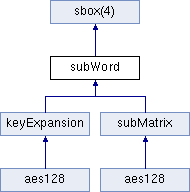
\includegraphics[width=0.4\textwidth, height=0.4\textheight, keepaspectratio]{./images/key_expansion/subWord.png}
	\caption{Sub Word}
	\label{fig:sub_word2}
\end{figure}

\subsubsection{Rcon}

\index{Rcon} \index{round constant}

\textsf{\small Questa funzione ricorsiva permette di generare delle costanti di round, attraverso questa formula:}

\begin{itemize}
	\item \textsf{\small il round\_constant(1) = 1.}
	\item \textsf{\small round\_constant(i) = $2 \cdot \text{round\_constant}(i - 1) \text{se round\_constant(i - 1) < 0x80}$}
	\item \textsf{\small round\_constant($2 \cdot \text{round\_constant(i - 1)}$) $ \oplus \hspace{0.3mm} \text{0x11B } \ge 0x80$ }
\end{itemize}

\subsection{I Rounds} %TODO: Rinominare in qualcos'altro.

\index{rounds} \index{mix columns}

\textsf{\small Dopo aver ottenuto le chiavi, vengono compiuti i vari rounds.} 

\textsf{\small Per ogni round, eseguiamo questi passaggi, tranne per l'ultimo dove non effettuiamo il passaggio delle \emph{Mix Columns}, perché non aumenterebbe la sicurezza e semplicemente rallenterebbe: } %TODO: [magari approfondire il perché rallenterebbe]

\index{sub bytes} \index{shift rows} \index{mix columns} \index{add round key} \index{confusione} \index{segretezza della chiave} \index{diffusione} \index{Shannon}

\begin{itemize}
	\item[] \textsf{\small Applichiamo il principio di \emph{confusione} attraverso il passaggio \emph{Sub-bytes}.}
	\item \textsf{\small \underline{\emph{Sub-bytes}}: Ogni byte viene mappato in un diverso byte attraverso una s-box. Questo step applica la proprietà di \emph{confusione} di Shannon, perché oscura la relazione tra ogni byte.}
	\item[] \textsf{\small Applichiamo la proprietà di \emph{diffusione}:}
	\item \textsf{\small \underline{\emph{Shift Rows}}: La seconda riga della matrice viene spostata di 1 verso sinistra. La terza riga di 2 posizioni e la quarta di 3 (sempre verso sinistra).}
	\item \textsf{\small \underline{\emph{Mix Columns}}: Ogni bit delle colonne della matrice (di stato) vengono mischiate.} %TODO: Approfondire come vengono mischiate
	\item[] \textsf{\small Applichiamo la proprietà di \emph{segretezza della chiave}:}
	\item \textsf{\small \underline{\emph{Add Round Key}}: Viene applicata la chiave del prossimo round attraverso uno XOR.} %TODO: applicata, meglio trovare un altro verbo
\end{itemize}

\begin{figure}[H] %TODO: Cambiare immagine?
	\centering
	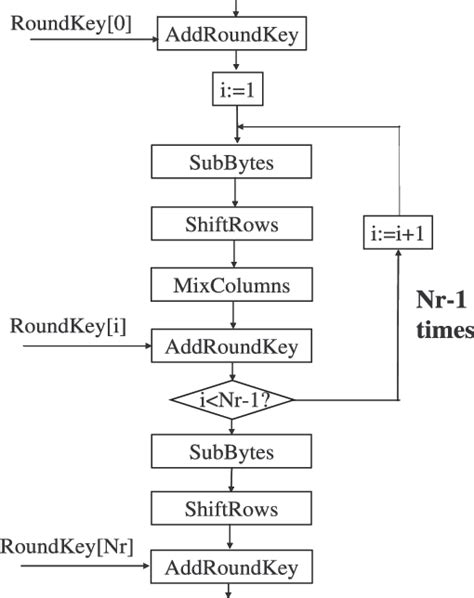
\includegraphics[width=0.5\textwidth, height=0.5\textheight, keepaspectratio]{./images/aes/flowcharts/aes_flowchart.png}
	\caption{AES Rounds Flowchart}
	\label{fig:aes_flowchart2}
\end{figure}

\index{rounds}

\textsf{\small Più rounds aggiungiamo, più sicurezza, ma questo porterebbe ad un rallentamento dell'algoritmo e quindi delle performance.}
\textsf{\small Per questo serve un compromesso tra sicurezza e prestazioni.}

\index{AES} \index{rounds}

\textsf{\small Quando AES era in sviluppo venne trovata una scorciatoia attraverso 6 rounds, per evitare ciò, sono stati aggiunti 4 rounds extra, come \emph{margine di sicurezza}.} %TODO: Quando AES era in sviluppo venne trovata una scorciatoia attraverso 6 rounds, [come possiamo notare ogni bit di output di un round dipende da ogni bit dei due rounds precedenti ] per evitare questo sono stati aggiunti 4 rounds extra, come \emph{margine di sicurezza}. %TODO: magari approfondire?

%TODO: [magari aggiungere qualche immagine sul procedimento]

%TODO: la subsection modalità di AES magari la sposto in un capitolo a parte? Oppure semplicemente ampio con le modalità di AES.

%TODO: subsection Add Round Key, Sub Bytes, Shift Rows, Mix Columns

\subsection{Add Round Key}

\index{add round key} \index{Galois} \index{XOR} \index{round} \index{matrice di stato}

\textsf{\small Viene aggiunto (ovvero nella matematica di Galois viene eseguito un'operazione di XOR) tra la matrice di stato (16 bytes = 4 words) e la chiave di round (anch'essa 16 bytes).}

\begin{figure}[H]
	\centering
	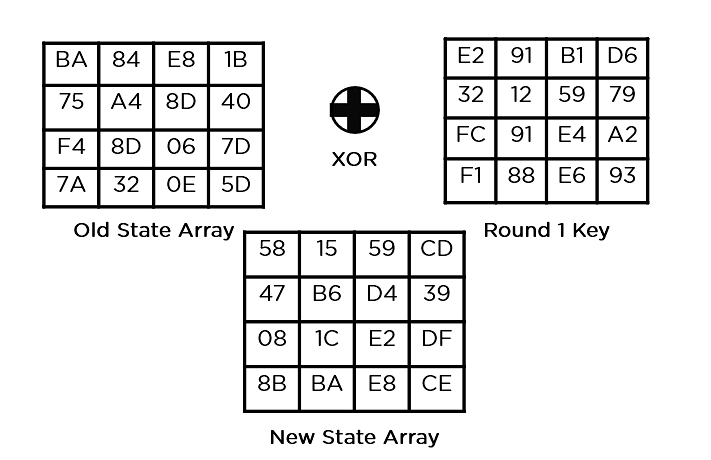
\includegraphics[width=0.7\textwidth, height=0.7\textheight, keepaspectratio]{./images/aes/add_round_key.png} %TODO: prima era roundkey.png
	\caption{Add Round Key}
	\label{fig:add_round_key2}
\end{figure}

%\vspace{-1.62cm}

\textsf{\small Per esempio, nell'immagine sopra, BA $ \oplus $ E2 = 58 $ \Leftrightarrow 10111010 \oplus 11100010 = 1011000 $.}

\subsection{Sub Bytes}

\index{sub bytes}

\textsf{\small Ognuno dei 16 bytes della matrice di stato viene sostituito con il corrispondente byte della S-BOX.}

\begin{figure}[H]
	\centering
	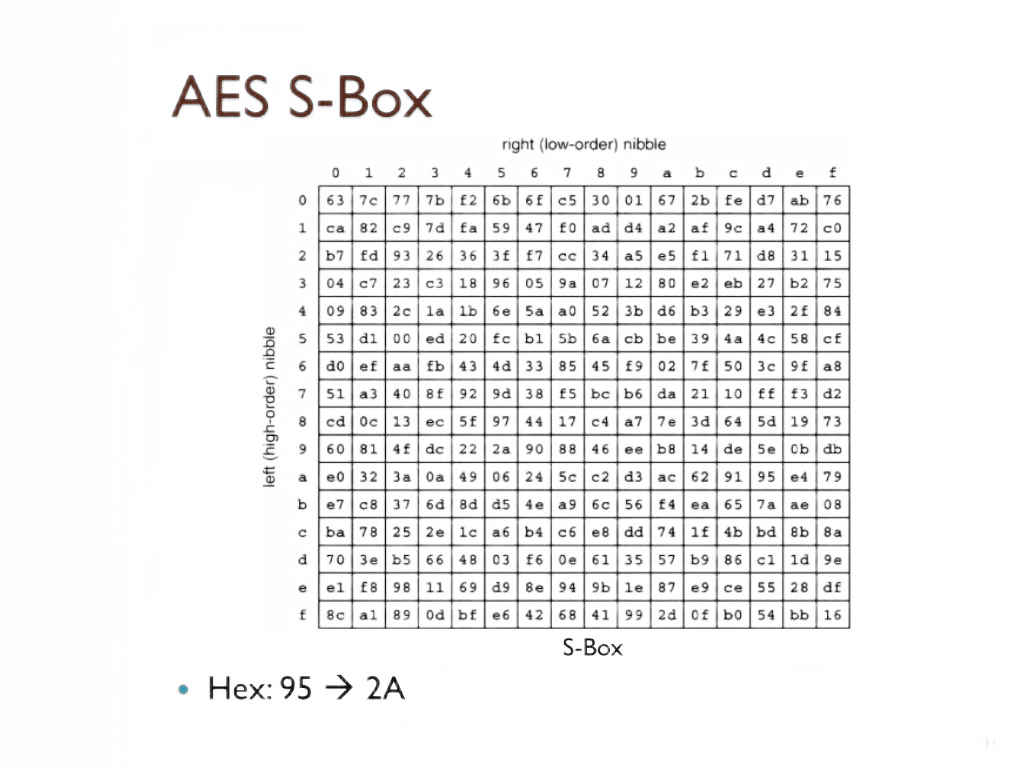
\includegraphics[width=.9\textwidth, height=.9\textheight, keepaspectratio]{./images/aes/aes-s-box-no-background.png}
	\caption{S-BOX}
	\label{fig:sbox}
\end{figure}

\textsf{\small Come si evince dall'esempio nell'immagine il valore 95, prendendo la nona riga e la quinta colonna, viene sostituito con il valore 2A.}

\subsection{Shift Rows}

\index{shift rows}

\textsf{\small Rotazione della seconda, terza e quarta riga.}

\begin{figure}[H]
	\centering
	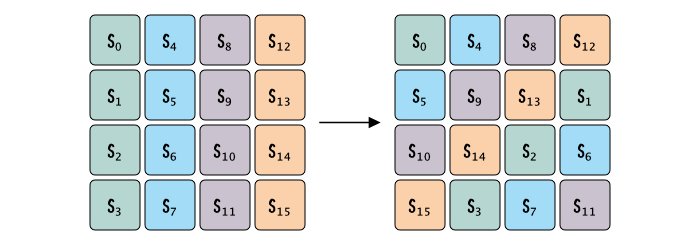
\includegraphics[width=.9\textwidth, height=.9\textheight, keepaspectratio]{./images/aes/aes-shift-rows.png}
	\caption{Shift Rows}
	\label{fig:shift_rows2}
\end{figure}

\begin{itemize}
	%\setlength\itemsep{1em} %TODO: remove
	\item \textsf{\small Shift della seconda riga di 1 posizione a sinistra.}
	\item \textsf{\small Shift della terza riga di 2 posizioni a sinistra.}
	\item \textsf{\small Shift della quarta riga di 3 posizioni a sinistra.}
\end{itemize}

\subsection{Mix Columns}

\index{mix columns} \index{matrice dello stato}

\textsf{\small Ogni byte viene della matrice dello stato è combinato usando una trasformazione lineare invertibile.}

\begin{figure}[H]
	\centering
	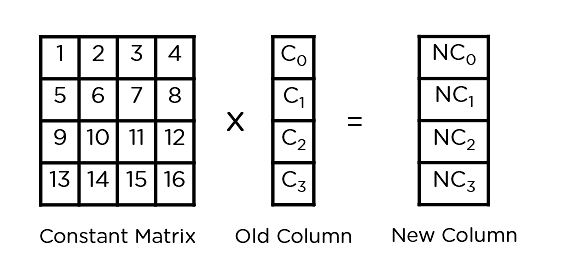
\includegraphics[width=.9\textwidth, height=.9\textheight, keepaspectratio]{./images/aes/mixcolumns.png}
	\caption{Mix Columns}
	\label{fig:mix_columns2}
\end{figure}

\textsf{\small Le equazioni per ricavare la nuova colonna: }

\textsf{\small $ NC_0 = galois\_multiplication 1 (C_0) \oplus galois\_multiplication 2 (C_1) \oplus C_2 \oplus C_3 $}

\textsf{\small $ NC_1 = C_0 \oplus galois\_multiplication 1 (C_1) \oplus galois\_multiplication 2 (C_2) \oplus C_3 $}

\textsf{\small $ NC_2 = C_0 \oplus C_1 \oplus galois\_multiplication 1 (C_2) \oplus galois\_multiplication 2 (C_3) $ }

\textsf{\small $ NC_3 = galois\_multiplication 2 (C_0) \oplus C_1 \oplus C_2 \oplus galois\_multiplication 1 (C_3) $}

\subsection{Le modalità di AES} %TODO: section/subsection: "Come può essere usato AES?" o "Con quali combinazioni può essere usato AES" o "In combinazione a cosa può essere usato AES"? o "Le modalità di AES"

\index{AES} \index{modalità}

\textsf{\small AES non può essere utilizzato così com'è, ma necessita di essere adoperato in combinazione a una modalità. } %TODO: AES non può essere usato così com'è, ma necessita di essere utilizzato in combinazione a una modalità .
\textsf{\small Una modalità è un sistema per trasformare l'efficacia di un algoritmo crittografico.} %TODO: processo/sistema/procedimento; aumentare/incrementare/trasformare/avanzare;

\index{AES} \index{ECB} \index{CBC} \index{CFB} \index{OFB} \index{CTR}

\textsf{\small Di seguito, alcune delle modalità di AES: }

\begin{itemize} %TODO: approfondirli, scrivere qualcosa di ciascuno
	\item \textsf{\small \textbf{ECB} (\emph{\textbf{E}lectronic \textbf{C}ode \textbf{B}ook})}
	\item \textsf{\small \textbf{CBC} (\emph{\textbf{C}ipher \textbf{B}lock \textbf{C}haining})}
	\item \textsf{\small \textbf{CFB} (\emph{\textbf{C}ipher \textbf{F}eed\textbf{B}ack)}}
	\item \textsf{\small \textbf{OFB} (\emph{\textbf{O}utput \textbf{F}eed\textbf{B}ack)}}
	\item \textsf{\small \textbf{CTR} (\emph{\textbf{C}oun\textbf{t}e\textbf{r} mode})}
	%\item \textsf{\small }
\end{itemize} 

%TODO: magari approfondire queste modalità oppure più tardi oppure scrivere giusto un filino per ognuna e poi al massimo lo riprendo dopo.

\newpage

\begin{comment}
\begin{figure}[H] %TODO: oppure mettere un'immagine sulle modalità, oppure mettere quueta prima delle modalità %TODO: remove visto che l'ho messo nel titolo?
	\centering
	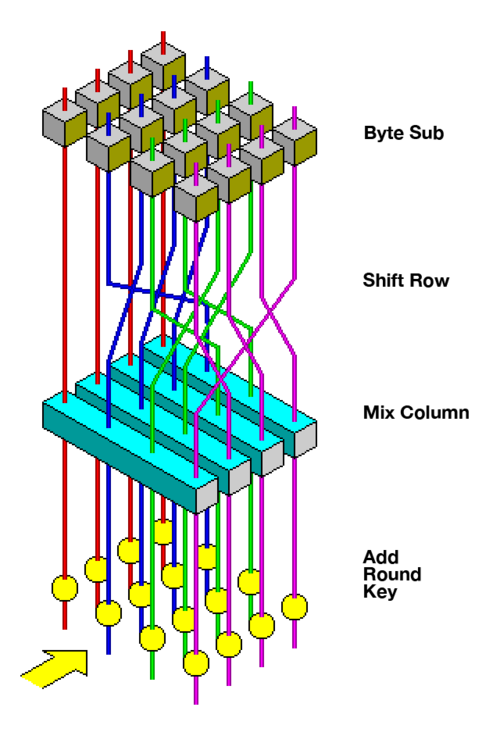
\includegraphics[width=0.6\textwidth, height=0.6\textheight, keepaspectratio]{./images/aes/500px-AES_(Rijndael)_Round_Function.png}
	\caption{AES Round Function}
	\label{fig:500px-AES_(Rijndael)_Round_Function}
\end{figure}
\end{comment}

%TODO: Approfondirli magari nella sezione dei pro e contro e dei possibili attacchi come: PA (Padding Attack), CPA (Chosen Plaintext Attack), CCA (Chosen Ci)

% -------------------------------- FINE CAPITOLO -------------------------------------- %TODO: oppure chiamarlo: "Meccanismo"/"Il Meccanismo"?
	
	% ================================ LA MATEMATICA DIETRO AES ============================

\chapter{La Matematica dietro AES}

%TODO: matrici 4x4
%TODO: Campo finito (campo di Galois). (p^n elementi)
%TODO: trasformazione affine invertibile.
%TODO: punto fisso (in matematica), punti fissi opposti.

%TODO: S-Box
%TODO: Rijndael Key Scheduler/AES Key Scheduler

%TODO: numero colonne = numero bit blocco in input / 32

% ======================================================================================


% ---------------------------- SECTION: INTRODUZIONE -----------------------------------

%\newpage

\section{Introduzione}

% ---------------------------- SECTION:  ----------------------------------

\newpage

\section{} 

% -------------------------------- FINE CAPITOLO ---------------------------------------
	
	% ================================ L'IMPLEMENTAZIONE ====================================

\chapter{L'implementazione}

%TODO: Implementazione in C++
%TODO: Con gui e command line o solo gui.

%TODO: Volendo anche Java?

%TODO: Presenterò/Mostrerò due implementazioni una fatta specificamente per questo progetto in C++ e un'altra in Java che avevo fatto per altri progetti.
%TODO: Quella in C++ sarà più completa rispetto di quella in Java.

% =======================================================================================

% ---------------------------- SECTION: INTRODUZIONE ------------------------------------

\section{Introduzione}

\textsf{\small In questo capitolo, presenterò due implementazioni, una elaborata esclusivamente per questo progetto in C++ e un'altra in Java che avevo creato per altri progetti universitari. Quella in C++ risulterà più completa rispetto a quella in Java.} %TODO: In questo capitolo, presenterò due implementazioni, una elaborata esclusivamente per questo progetto in C++ e un'altra in Java che avevo creato per altri progetti universitari. Quella in C++ risulterà più completa rispetto a quella in Java.

% ---------------------------- SECTION: IMPLEMENTAZIONE IN C++ --------------------------

\section{Implementazione in C++}

\textsf{\small Ho adottato C++23 per questo progetto. In esso sono presenti una interfaccia grafica e una applicazione da linea di comando, entrambe hanno le stesse operazioni.} %TODO: Ho adottato C++23 per questo progetto. In esso sono presenti una interfaccia grafica e una applicazione da linea di comando, entrambe hanno le stesse operazioni.

\textsf{\small Inanzittutto, esibirò, le funzioni riguardanti la matematica di Galois di cui mi sono avvalso.}

%TODO: Inanzittutto, esibirò, le funzioni riguardanti la matematica di Galois di cui mi sono avvalso.

\subsection{Matematica di Galois}

\begin{figure}[H]
	\centering
	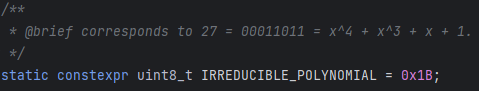
\includegraphics[width=1\textwidth, height=1\textheight, keepaspectratio]{./images/code/cpp/galois_math/irreducible_polynomial.PNG}
	\caption{Polinomio irriducibile}
	\label{fig:irreducible_polynomial}
\end{figure}

\textsf{\small Riguardo alla matematica nel campo di Galois, ho adoperato tre funzioni: una che implementa l'addizione e la sottrazione, una per la moltiplicazione e una per generare le costanti di round.} %TODO: 

\textsf{\small Nel campo di Galois, sia l'addizione che la sottrazione sono semplicemente un'operazione di XOR. Questa funzione prende due parametri x ed y di tipo \emph{uint8\_t} (che corrisponde a un \emph{unsigned char}) e restituisce lo XOR tra essi.}

\begin{figure}[H]
	\centering
	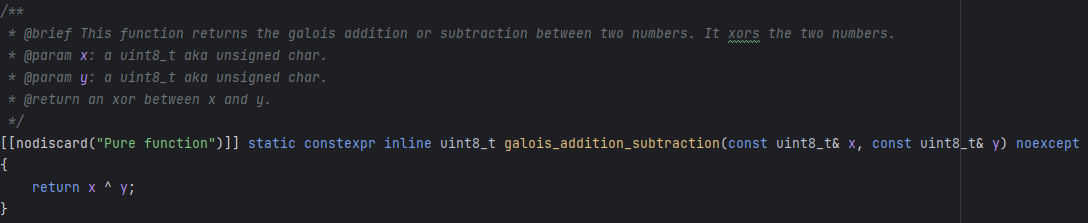
\includegraphics[width=1\textwidth, height=1\textheight, keepaspectratio]{./images/code/cpp/galois_math/galois_addition_subtraction.PNG}
	\caption{Addizione e sottrazione nel campo di Galois}
	\label{fig:galois_addition_subtraction}
\end{figure}

\textsf{\small \emph{galois\_multiplication()} prende due \emph{uint8\_t} come parametri e restituisce la moltiplicazione tra questi nel campo di Galois.}

\textsf{\emph{static constexpr} indicano che la funzione può essere eseguita a compile time. \emph{noexcept} indica che la funziona non lancia eccezioni. \emph{[[nodiscard]]} indica che il risultato che viene restituito non può essere ignorato, ma deve essere utilizzato.}

%TODO: Aggiungere reference alla parte nel capitolo della Matematica o aggiungere breve spiegazione.

\textsf{\small Facciamo un loop su ogni bit del byte e verifichiamo se il secondo valore \emph{y} ha il bit meno significativo attivo (y \& 0x01) allora aggiungiamo \emph{x} (ovvero eseguiamo uno XOR) al risultato. Dopodiché verifichiamo se il bit più significativo \emph{high\_bit} è attivo in \emph{x}. Poi ruotiamo x di 1. Se l'\emph{high\_bit} è \emph{true} eseguiamo uno XOR tra x e il polinomio irriducibile \emph{IRREDUCIBLE\_POLYNOMIAL}, ovvero $0x1\text{B}$. Infine ruotiamo il secondo valore di 1 per ruotarlo a destra. Poi restituiamo il risultato finale delle operazioni.}

\begin{figure}[H]
	\centering
	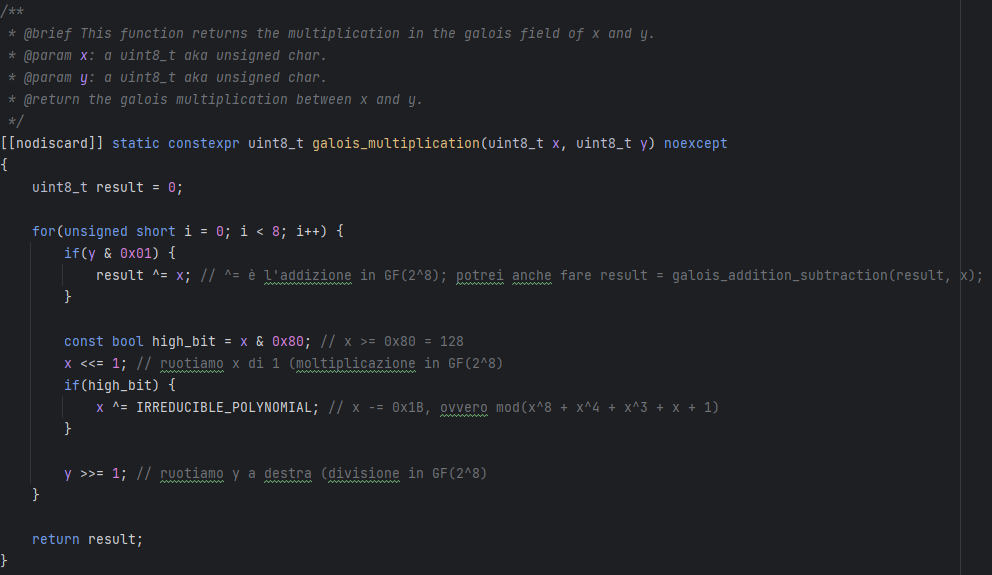
\includegraphics[width=1\textwidth, height=1\textheight, keepaspectratio]{./images/code/cpp/galois_math/galois_multiplication.PNG}
	\caption{Moltiplicazione nel campo di Galois}
	\label{fig:galois_multiplication}
\end{figure}

\textsf{\small \emph{round\_constant\_generator(const uint8\_t\& x)} prende un numero in input e restituisce la round constant.} %TODO:

\textsf{\small Questa funzione è utilizzata per generare la round constant.}
\textsf{\small L'algoritmo di questa funzione è il seguente: }

\begin{itemize}
	\item \textsf{\small il round\_constant(1) = 1.}
	\item \textsf{\small round\_constant(i) = $2 \cdot \text{round\_constant}(i - 1) \text{se round\_constant(i - 1) < 0x80}$}
	\item \textsf{\small round\_constant($2 \cdot \text{round\_constant(i - 1)}$) $ \oplus \hspace{0.3mm} \text{0x11B } \ge 0x80$ }
\end{itemize}

\begin{figure}[H] %TODO: update.
	\centering
	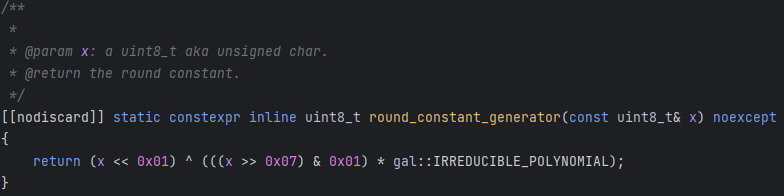
\includegraphics[width=1\textwidth, height=1\textheight, keepaspectratio]{./images/code/cpp/galois_math/round_constant_generator.PNG}
	\caption{Generatrice delle costanti di round}
	\label{fig:round_constant_generator}
\end{figure}

%TODO: Come prima cosa mostrerò l'implementazione dell'algoritmo di AES con tutte le varie operazioni all'interno di ogni round di AES, ovvero: add round key, sub bytes, shift rows e mix columns. Dopodiché presenterò la parte di Key Expansion, ovvero come vengono ottenute le chiavi per ogni round, anch'esso composto da queste fasi: rot word, sub word, rcon.

%\subsection{Cifratura} %TODO: uncomment?

\subsection{Add Round Key}

\textsf{\small Nella fase di \emph{add\_round\_key()} la chiave di round viene aggiunta alla matrice di stato.}

\textsf{\small La funzione prende la matrice di stato 4x4 (formata da due std::array di grandezza BLOCK\_WORDS che indica il numero di words in un blocco, ovvero 4) e la chiave del round come puntatore e le aggiunge.}

\begin{figure}[H]
	\centering
	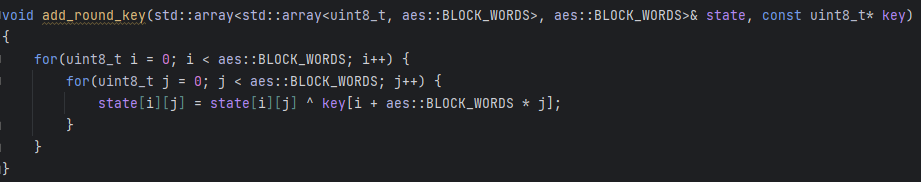
\includegraphics[width=1\textwidth, height=1\textheight, keepaspectratio]{./images/code/cpp/encryption/add_round_key.PNG}
	\caption{Add Round Key}
	\label{fig:add_round_key}
\end{figure}

\subsection{Sub Bytes}

\textsf{\small Nella funzione \emph{sub\_bytes} ogni byte della matrice di stato viene sostituito con quelli presenti nella S-BOX.}

\textsf{\small Quindi, nella funzione viene passata la matrice di stato come reference, quindi tutti le modifiche verranno applicate anche all'esterno della funzione e poi viene eseguito un loop e ogni elemento viene sostituito con il corrispettivo della S-BOX.}

\begin{figure}[H]
	\centering
	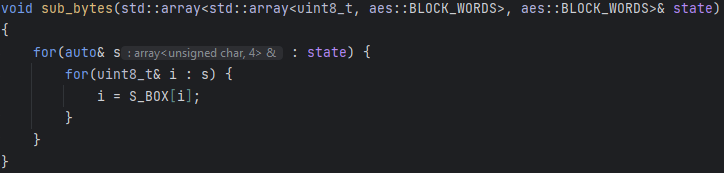
\includegraphics[width=1\textwidth, height=1\textheight, keepaspectratio]{./images/code/cpp/encryption/sub_bytes.PNG}
	\caption{Sub Bytes}
	\label{fig:sub_bytes}
\end{figure}

\subsection{Shift Rows}

\textsf{\small Nel passaggio di \emph{shift rows} le righe della matrice di stato verranno \emph{shiftate} di una posizione la seconda riga, di due posizione la terza e di tre la quarta.}

\textsf{\small Per fare questo ci avvaliamo di due funzioni, una \emph{shift\_row} per shiftare effettivamente le righe e nell'altra \emph{shift\_rows} per chiamare la precedente funzione per shiftare delle posizioni stabilite.}

%TODO: aggiungere altro?

\begin{figure}[H]
	\centering
	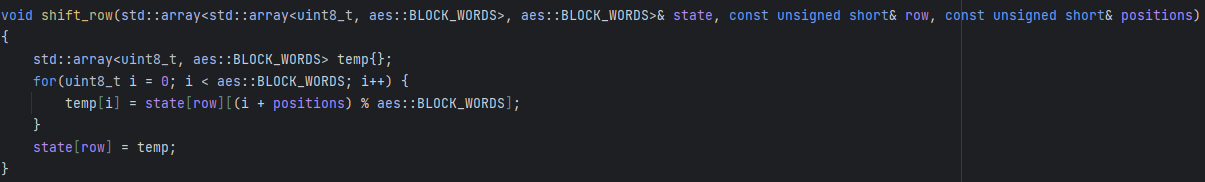
\includegraphics[width=1\textwidth, height=1\textheight, keepaspectratio]{./images/code/cpp/encryption/shift_row.PNG}
	\caption{Shift Row}
	\label{fig:shift_row}
\end{figure}

\textsf{\small } %TODO:

\begin{figure}[H]
	\centering
	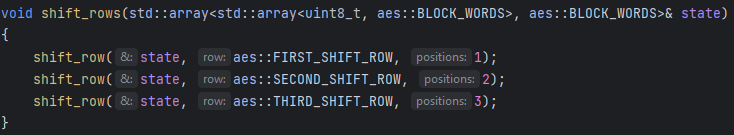
\includegraphics[width=1\textwidth, height=1\textheight, keepaspectratio]{./images/code/cpp/encryption/shift_rows.PNG}
	\caption{Shift Rows}
	\label{fig:shift_rows}
\end{figure}

\subsection{Mix Columns}

\textsf{\small La procedura \emph{mix\_columns} prende in input la matrice di stato, mescola i suoi bytes.} %TODO:

%TODO: Aggiungere altro.

\begin{figure}[H]
	\centering
	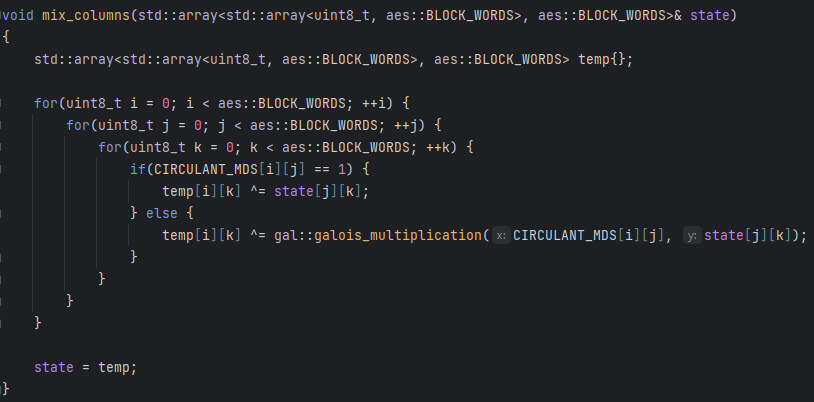
\includegraphics[width=1\textwidth, height=1\textheight, keepaspectratio]{./images/code/cpp/encryption/mix_columns.PNG}
	\caption{Mix Columns}
	\label{fig:mix_columns}
\end{figure}

%TODO: funzioni di decifrazione?

\subsection{Key Expansion}

\textsf{\small In questa funzione vengono generate le altre chiavi dei rounds a partire dalla prima chiave. Gli viene passata un array con la chiave, una word e la tipologia di AES: 128, 192 o 256.} %TODO:

\textsf{\small Dopodiché eseguiamo le operazioni di: \emph{rot\_word}, \emph{sub\_word}, e \emph{rcon}. Dopodiché viene eseguito uno XOR tra la chiave e il rcon. Dopodiché si continua a eseguire uno XOR con le chiavi precedenti.}

%TODO: Aggiungere altro.

\begin{figure}[H]
	\centering
	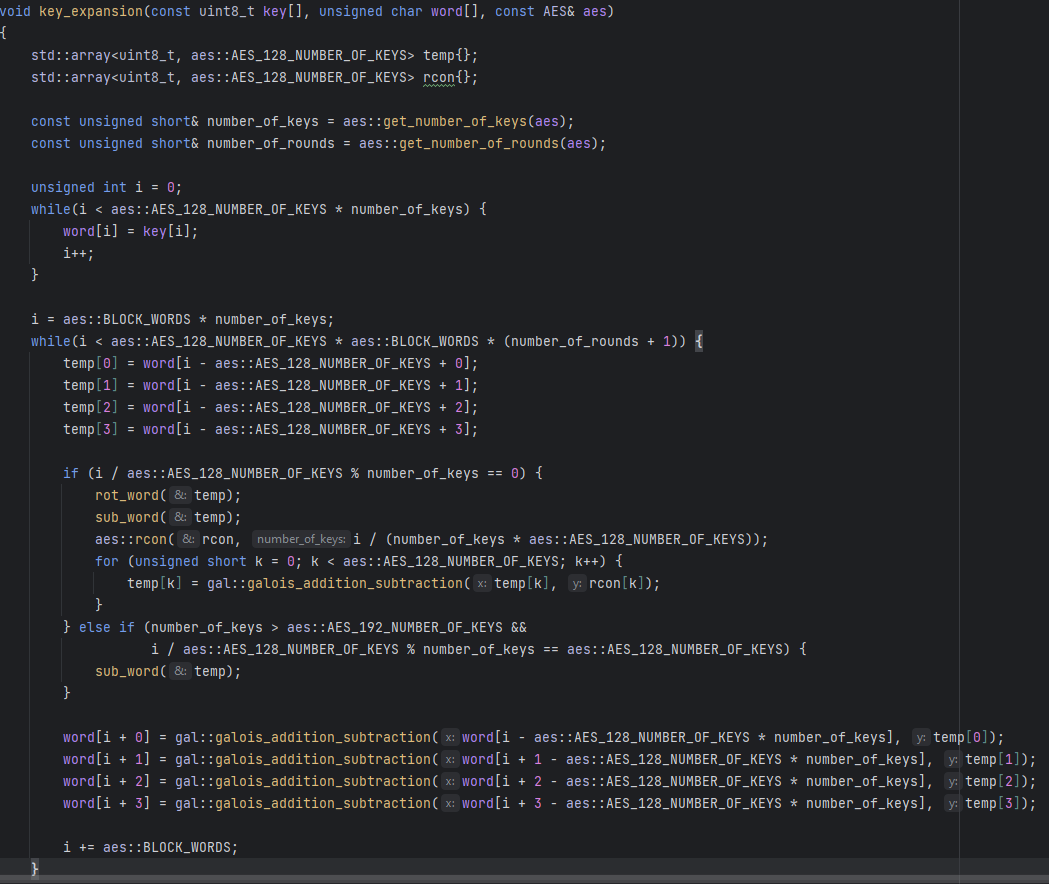
\includegraphics[width=1\textwidth, height=1\textheight, keepaspectratio]{./images/code/cpp/key_expansion/key_expansion.PNG}
	\caption{Key Expansion}
	\label{fig:key_expansion_code}
\end{figure}

\subsubsection{Rot Word}

\begin{figure}[H]
	\centering
	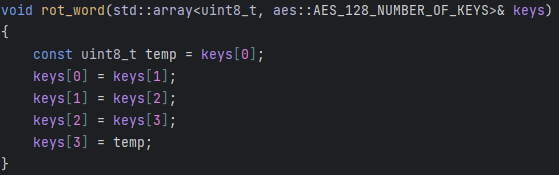
\includegraphics[width=1\textwidth, height=1\textheight, keepaspectratio]{./images/code/cpp/key_expansion/rot_word.PNG}
	\caption{Rot Word}
	\label{fig:rot_word}
\end{figure}

\textsf{\small In questa operazione ogni byte (word di 32 bits, ovvero 4 bytes) viene ruotato di 1 posizione.} %TODO: Aggiungere altro.

\subsubsection{Sub Word}

\begin{figure}[H]
	\centering
	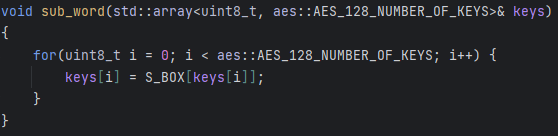
\includegraphics[width=1\textwidth, height=1\textheight, keepaspectratio]{./images/code/cpp/key_expansion/sub_word.PNG}
	\caption{Sub Word}
	\label{fig:sub_word}
\end{figure}

\textsf{\small Nella procedura \emph{sub\_word()} ogni byte della chiave viene sostituita con quella della S-BOX.} %TODO:

\subsubsection{Rcon}

\begin{figure}[H]
	\centering
	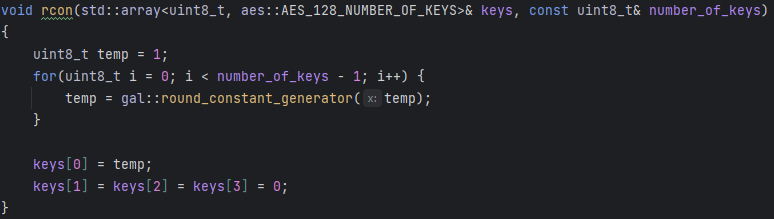
\includegraphics[width=1\textwidth, height=1\textheight, keepaspectratio]{./images/code/cpp/key_expansion/rcon.PNG}
	\caption{Rcon}
	\label{fig:rcon}
\end{figure}

\textsf{\small Nella funzione \emph{rcon}, le \emph{round constants} vengono generate attraverso una funzione ricorsiva.} %TODO:

\subsubsection{Xor Blocks} %TODO: uncomment?

\textsf{\small Con questa funzione eseguiamo uno XOR per ogni bit \emph{i} tra i blocchi x e y e assegniamo il risultato a ogni bit del blocco z. }

\textsf{\small Il loop viene eseguito in base alla grandezza del blocco.}

\begin{figure}[H]
	\centering
	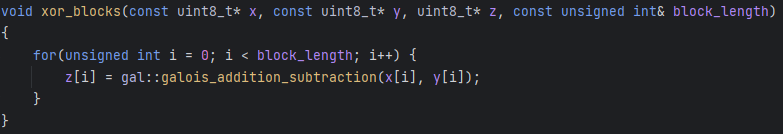
\includegraphics[width=1\textwidth, height=1\textheight, keepaspectratio]{./images/code/cpp/key_expansion/xor_blocks.PNG}
	\caption{Xor Blocks}
	\label{fig:xor_blocks}
\end{figure}

%\textsf{\small } %TODO:

\subsection{Modes}

\textsf{\small } %TODO:

%TODO: subsection: Modes con codice? Questo si potrebbe fare.

\subsubsection{ECB}

\textsf{\small ECB è la modalità più semplice e anche quella che non dovrebbe mai essere usata.} %TODO: aggiungere reference alla spiegazione della modalità.

\textsf{\small In questa modalità, semplicemente, ogni blocco viene cifrato com'è. Nessun vettore di inizializzazione viene utilizzato. Lo stesso input genererà lo stesso identico output.}

\textsf{\small Questa modalità inoltre accetta solo blocchi divisibili per 16, questo viene garantito attraverso la funzione \emph{verify\_length()} che verifica e lancia un'eccezione altrimenti.}

\begin{figure}[H]
	\centering
	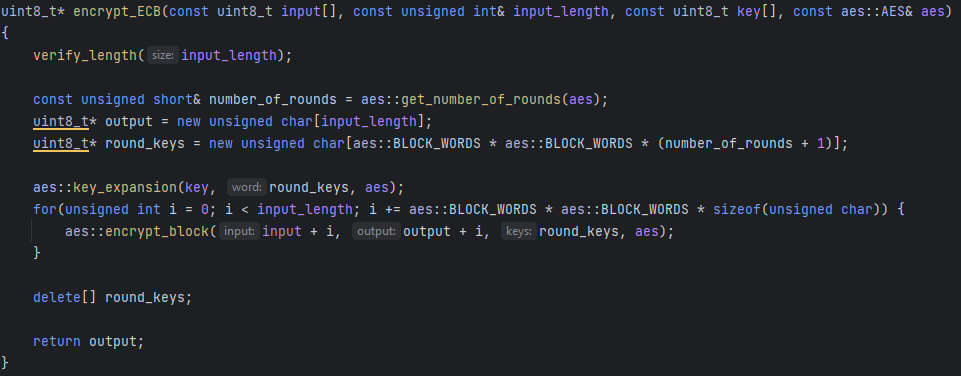
\includegraphics[width=1\textwidth, height=1\textheight, keepaspectratio]{./images/code/cpp/modes/encrypt_ECB.PNG}
	\caption{Cifratura ECB}
	\label{fig:encrypt_ECB}
\end{figure}

\textsf{\small Per la decifrazione è lo stesso procedimento, ma inverso. } %TODO:

\begin{figure}[H]
	\centering
	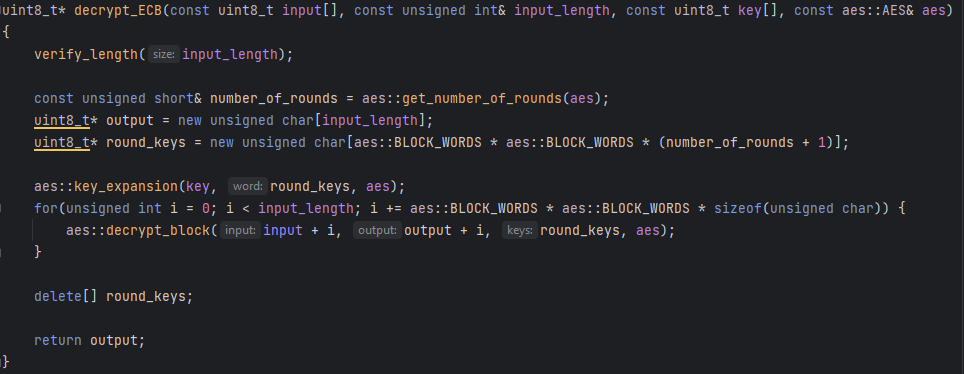
\includegraphics[width=1\textwidth, height=1\textheight, keepaspectratio]{./images/code/cpp/modes/decrypt_ECB.PNG}
	\caption{Decifrazione ECB}
	\label{fig:decrypt_ECB}
\end{figure}

\subsubsection{CBC}

\textsf{\small CBC è la modalità di chaining, in cui viene utilizzato un IV (initialization vector) per aggiungere casualità e viene eseguito uno XOR tra il messaggio in chiaro e il testo cifrato.} %TODO:

\begin{figure}[H]
	\centering
	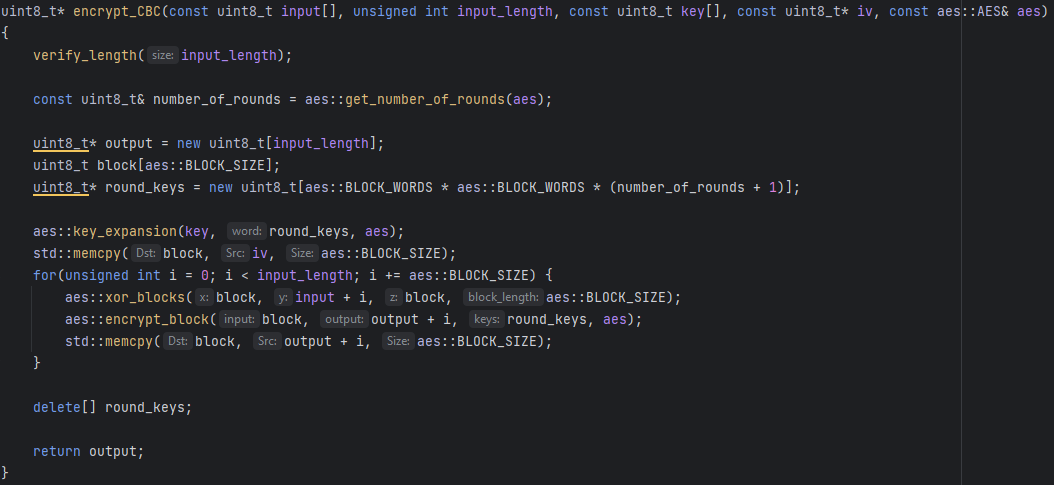
\includegraphics[width=1\textwidth, height=1\textheight, keepaspectratio]{./images/code/cpp/modes/encrypt_CBC.PNG}
	\caption{Cifratura CBC}
	\label{fig:encrypt_CBC}
\end{figure}

\textsf{\small } %TODO:

\begin{figure}[H]
	\centering
	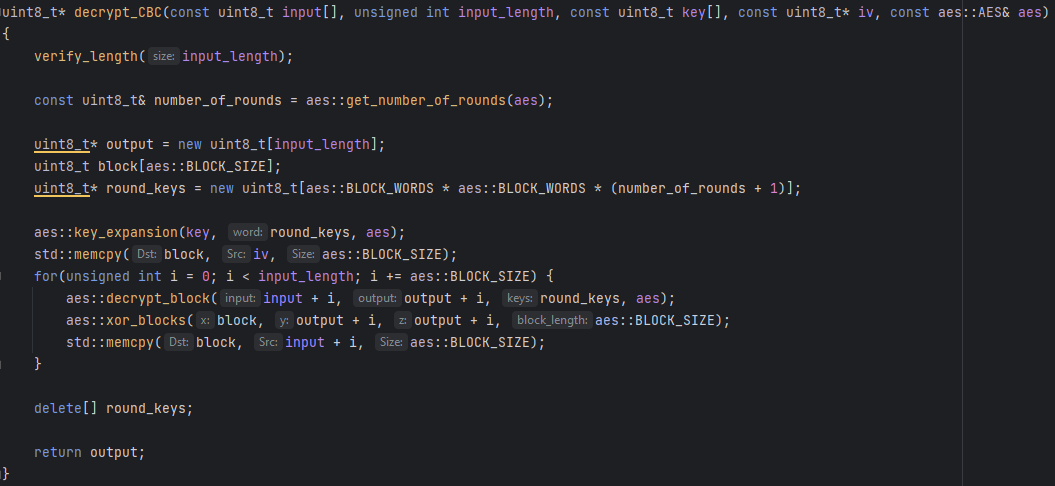
\includegraphics[width=1\textwidth, height=1\textheight, keepaspectratio]{./images/code/cpp/modes/decrypt_CBC.PNG}
	\caption{Decifrazione CBC}
	\label{fig:decrypt_CBC}
\end{figure}

\subsubsection{CFB}

\textsf{\small In queste funzioni, innanzitutto, verifico che la lunghezza dell'input sia divisibile per 16, poi ottengo il numero di rounds in base a quale AES stiamo utilizzando. Imposto l'output, il blocco, il blocco cifrato e le chiavi di rounds che ottengo dalla key\_expansion. Dopodiché cifro il blocco, eseguo uno XOR tra il plaintext e il blocco cifrato. Infine restituisco l'output.} %TODO:

\begin{figure}[H]
	\centering
	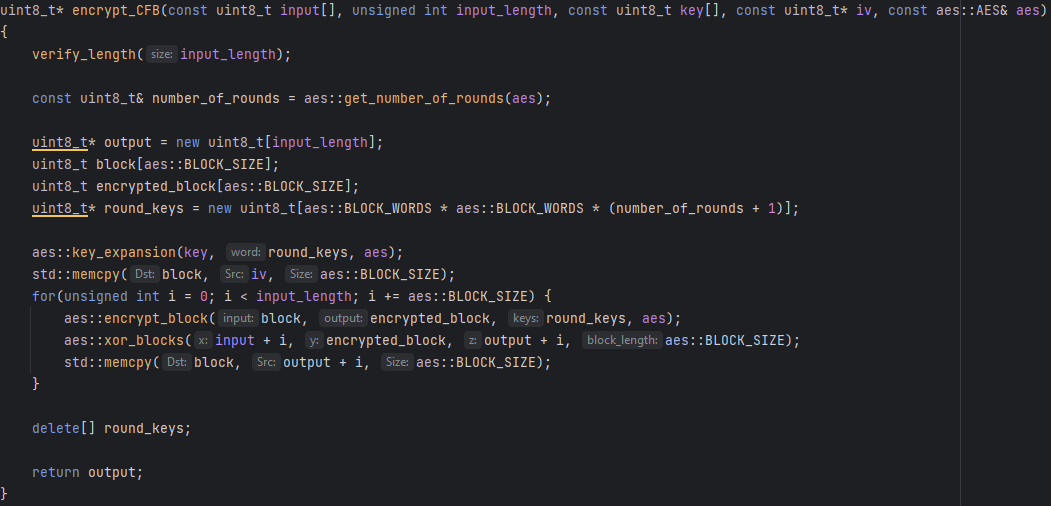
\includegraphics[width=1\textwidth, height=1\textheight, keepaspectratio]{./images/code/cpp/modes/encrypt_CFB.PNG}
	\caption{Cifratura CFB}
	\label{fig:encrypt_CFB}
\end{figure}

\textsf{\small }

\begin{figure}[H]
	\centering
	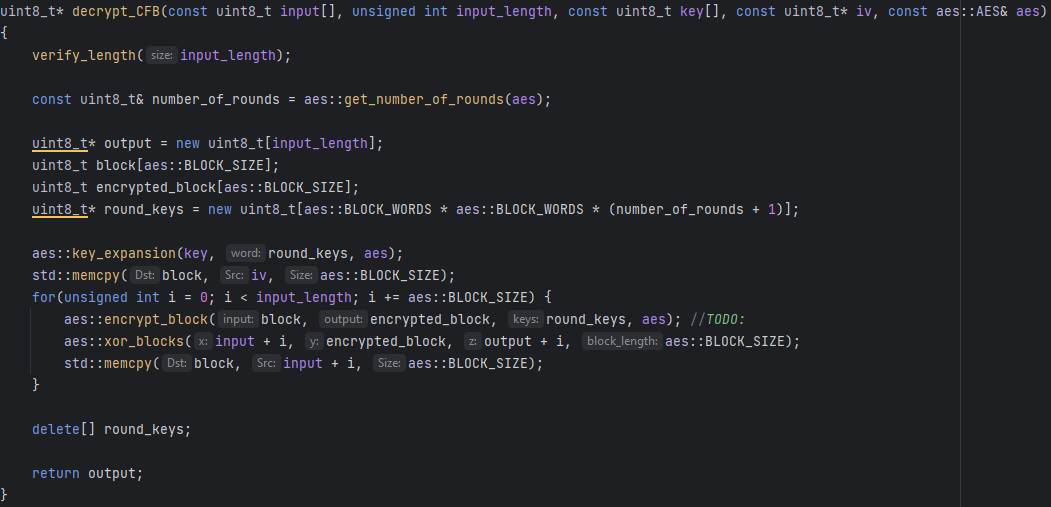
\includegraphics[width=1\textwidth, height=1\textheight, keepaspectratio]{./images/code/cpp/modes/decrypt_CFB.PNG}
	\caption{Decifrazione CFB}
	\label{fig:decrypt_CFB}
\end{figure}

\subsection{Paddings}

\textsf{\small Il padding viene utilizzato per aggiungere dei caratteri prestabiliti alla fine di un messaggio. Abbiamo due funzioni, una per aggiungere il padding, add\_padding e una per rimuoverlo, remove\_padding. Entrambe queste funzioni richiedono il messaggio da cui vogliamo aggiungere/rimuovere il padding e quale tipologia di padding applicare.} %TODO:

\textsf{\small Otteniamo, innanzitutto, il resto per vedere se il messaggio è perfettamente divisibile del BLOCK\_SIZE, ovvero 16 oppure no. Dopodiché calcoliamo la lunghezza mancante, sottraendo il BLOCK\_SIZE al resto.}

\begin{figure}[H]
	\centering
	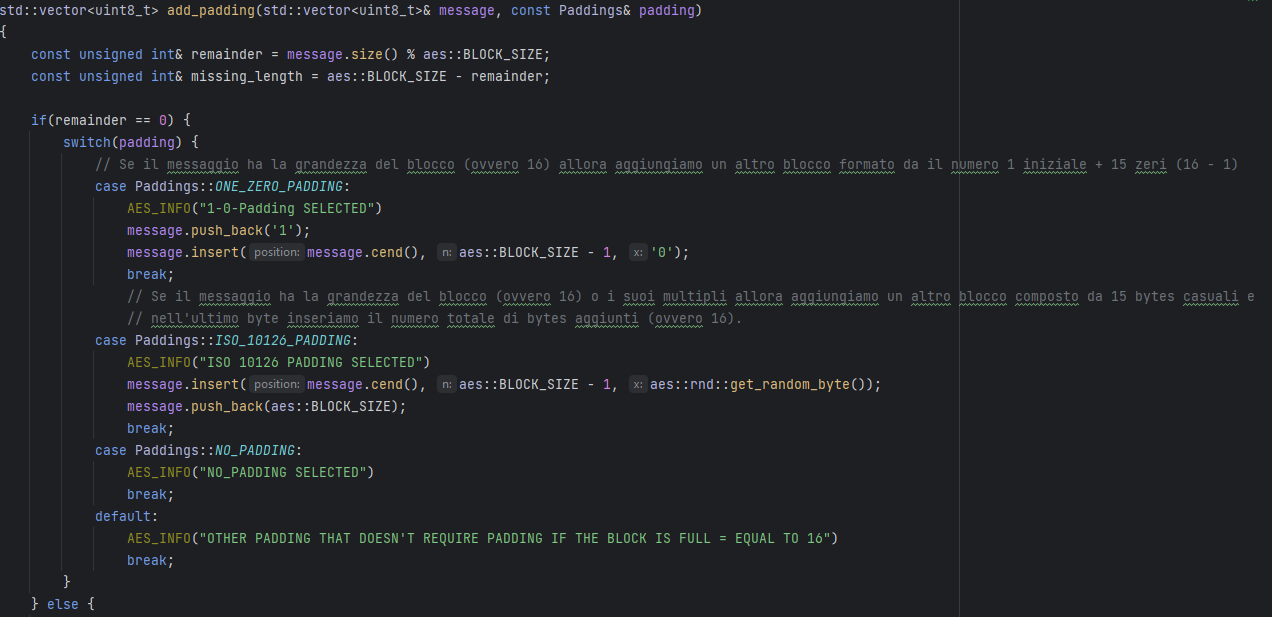
\includegraphics[width=1\textwidth, height=1\textheight, keepaspectratio]{./images/code/cpp/padding/add_padding0.PNG}
	\caption{Aggiunta del padding (1/2)}
	\label{fig:add_padding0}
\end{figure}

\textsf{\small Se il resto è 0, ovvero il blocco è formato da esattamente 16 caratteri, allora eseguiamo questo:}

\begin{itemize}
	\item \textsf{\small \textbf{1-0-Padding}: Aggiungiamo un ulteriore blocco di lunghezza 16, ove il primo elemento è il carattere '1' e il rimanente è composto da zeri.}
	\item \textsf{\small \textbf{ISO\_10126\_PADDING}: Aggiungiamo 15 caratteri casuali e nell'ultimo carattere inseriamo il numero di caratteri casuali aggiunti.}
	\item \textsf{\small \textbf{NO\_PADDING} o qualsiasi altro padding: non facciamo nulla.}
\end{itemize}

\begin{figure}[H]
	\centering
	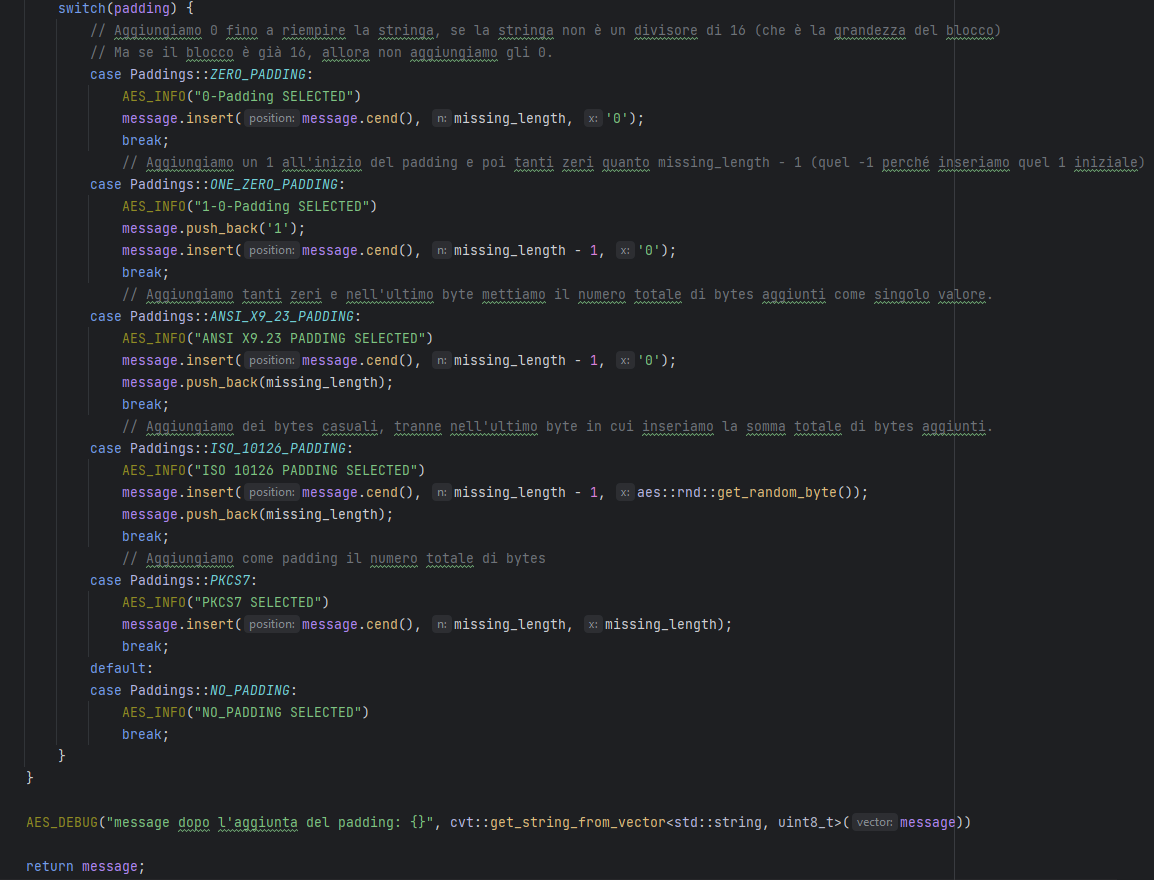
\includegraphics[width=1\textwidth, height=1\textheight, keepaspectratio]{./images/code/cpp/padding/add_padding1.PNG}
	\caption{Aggiunta del padding (2/2)}
	\label{fig:add_padding1}
\end{figure}

\textsf{\small Se il resto non è pari a 0, quindi il blocco non è pieno, non corrisponde a 16, allora eseguiamo:}

\begin{itemize}
	\item \textsf{\small \textbf{0-Padding}: Aggiungiamo tanti zeri quanti necessari per riempire il blocco.}
	\item \textsf{\small \textbf{1-0-Padding}: Aggiungiamo un 1 e poi tanti zeri quanti necessari per riempire il blocco.}
	\item \textsf{\small \textbf{ANSI\_X9\_23\_PADDING}: Aggiungiamo tanti zeri quanti necessari per riempire il blocco - 1, perché nell'ultimo byte inseriamo il numero degli zeri che abbiamo aggiunto.}
	\item \textsf{\small \textbf{ISO\_10126\_PADDING}: Aggiungiamo dei numeri casuali fino a riempire il blocco - 1, tranne che nell'ultimo byte in cui inseriamo il numero di bytes casuali aggiunti.}
	\item \textsf{\small \textbf{PKCS7}: Aggiungiamo il numero di bytes che mancano al riempire il blocco in tutti i blocchi rimanenti.}
	\item \textsf{\small \textbf{NO\_PADDING}: Non eseguiamo alcuna operazione al testo in chiaro.}
\end{itemize}

\begin{figure}[H]
	\centering
	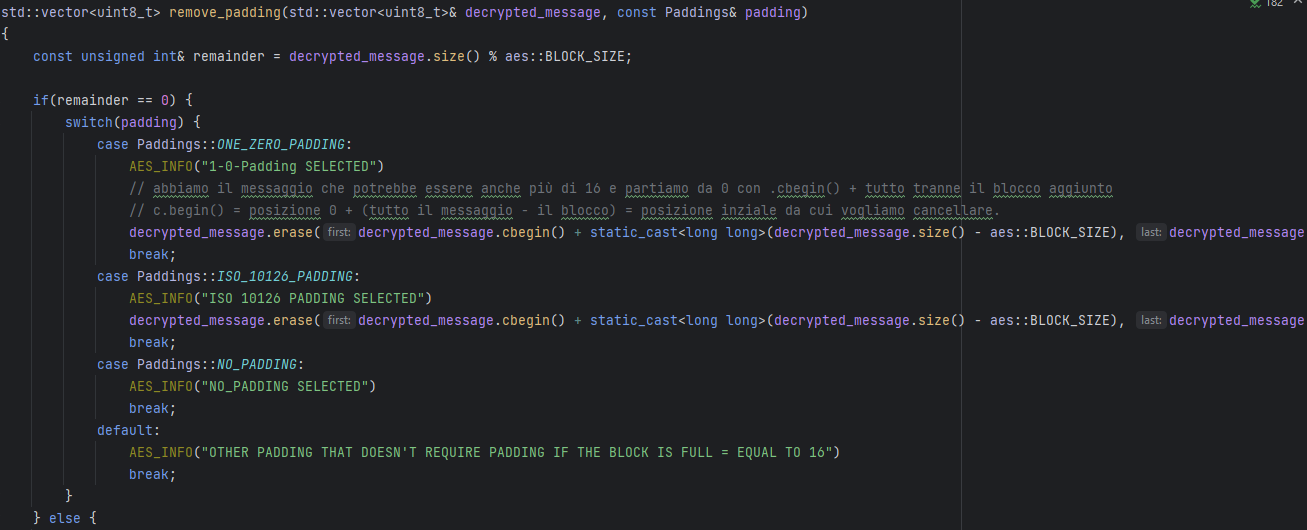
\includegraphics[width=1\textwidth, height=1\textheight, keepaspectratio]{./images/code/cpp/padding/remove_padding0.PNG}
	\caption{Rimozione del padding (1/2)}
	\label{fig:remove_padding0}
\end{figure}

\begin{figure}[H]
	\centering
	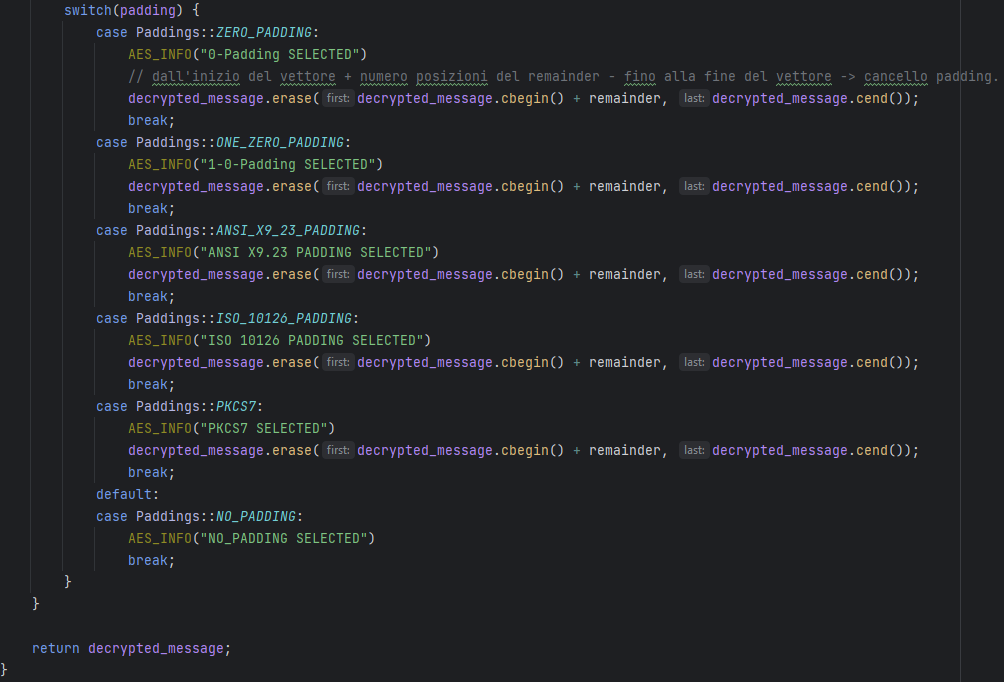
\includegraphics[width=1\textwidth, height=1\textheight, keepaspectratio]{./images/code/cpp/padding/remove_padding1.PNG}
	\caption{Rimozione del padding (2/2)}
	\label{fig:remove_padding1}
\end{figure}

\textsf{\small Per quanto riguarda la rimozione del padding, dal testo decifrato, è la stessa identica operazione dell'aggiunta, ma all'inverso, rimuovendo i bytes che avevamo aggiunto.} %TODO:

\subsection{API}

\textsf{\small Per poter interfacciarsi con tutte queste funzioni, ne sono presenti due: \emph{encrypt()} e \emph{decrypt()} che richiedono entrambe il messaggio (cifrato o in chiaro), la chiave, l'eventuale IV, opzionale, perché potrebbe non essere presente se si utilizza la modalità ECB, la tipologia di padding, la modalità e infine quale tipologia di AES.}

\subsubsection{Cifratura}

\textsf{\small Nella cifratura, viene aggiunto il padding chiamando \emph{add\_padding()} al messaggio in chiaro. Dopodiché, in base alla modalità scelta, viene restituito il messaggio cifrato.}

\begin{figure}[H]
	\centering
	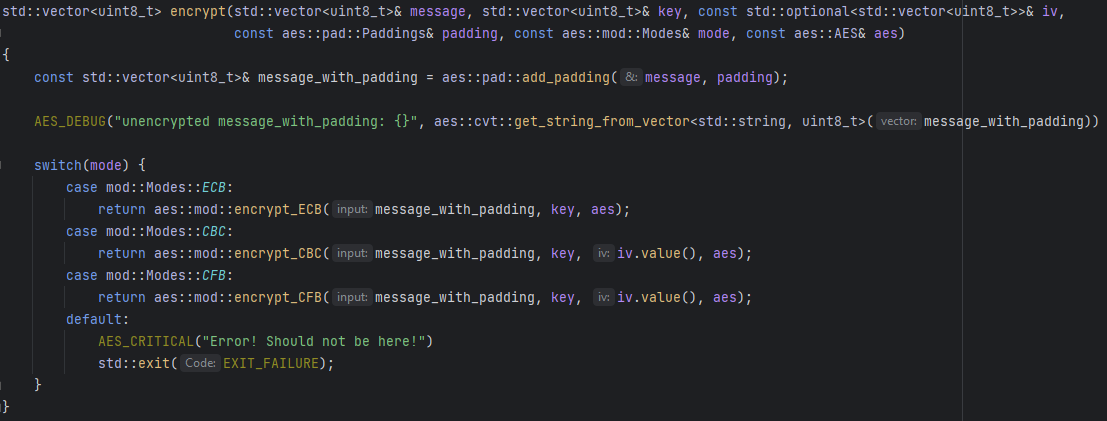
\includegraphics[width=1\textwidth, height=1\textheight, keepaspectratio]{./images/code/cpp/api/encrypt.PNG}
	\caption{Cifratura}
	\label{fig:encrypt}
\end{figure}

%TODO: encrypt_file?

\subsubsection{Decifratura}

\textsf{\small Nella decifratura, viene decifrato il messaggio in base alla modalità selezionata e dopodiché viene restituito il messaggio dopo la rimozione del padding, se presente.}

\begin{figure}[H]
	\centering
	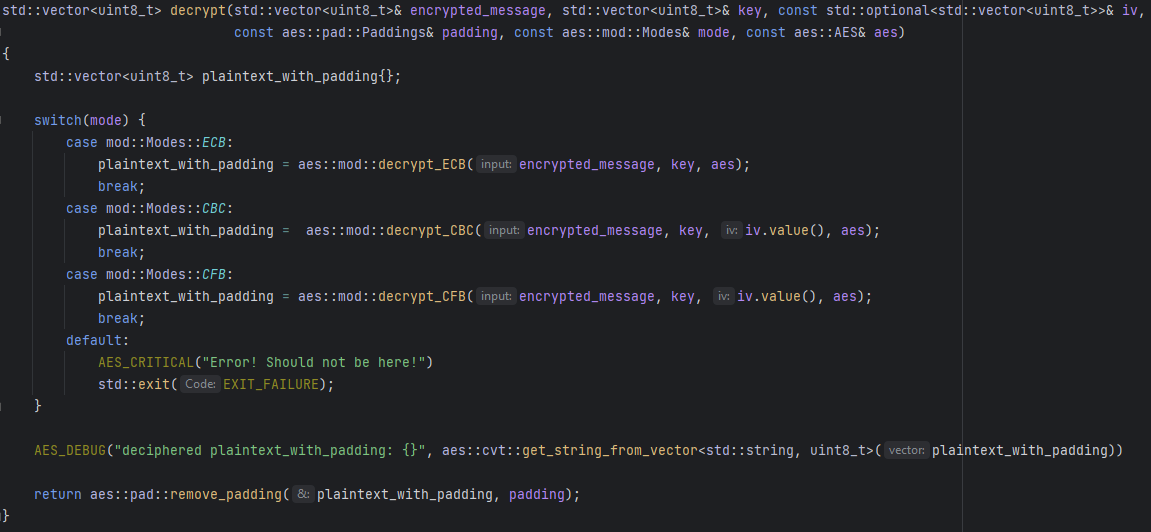
\includegraphics[width=1\textwidth, height=1\textheight, keepaspectratio]{./images/code/cpp/api/decrypt.PNG}
	\caption{Decifratura}
	\label{fig:decrypt}
\end{figure}

%TODO: decrypt_file?

%\textsf{\small } %TODO:

% ---------------------------- SECTION: IMPLEMENTAZIONE IN JAVA -------------------------

\section{Implementazione in Java}

\textsf{\small Per l'implementazione in Java, mi sono avvalso di Java 11 e ho usufruito delle librerie standard.} %TODO: 

\textsf{\small Ho definito, innanzitutto, delle variabili membro statiche, per definire la grandezza della chiave, quale algoritmo utilizzare, quale tipo di padding usufruire e altre inerenti l'iv e la salatura della password.}

\begin{figure}[H]
	\centering
	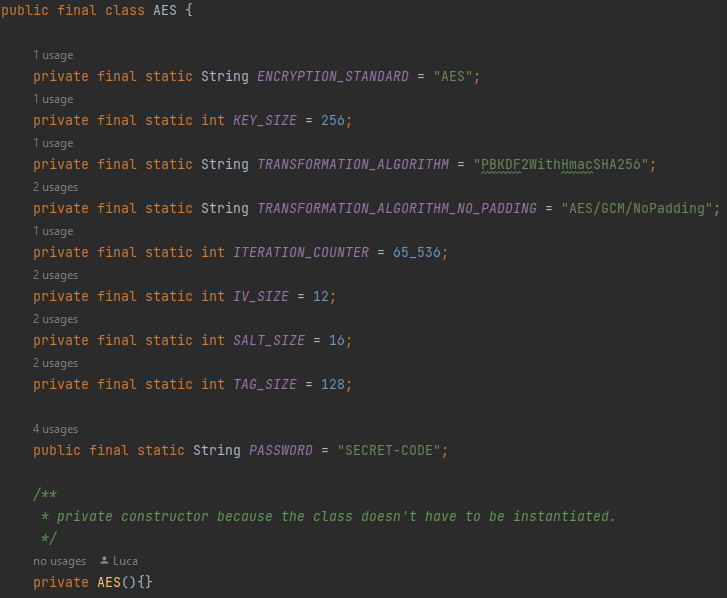
\includegraphics[width=1\textwidth, height=1\textheight, keepaspectratio]{./images/code/java/constructor_and_member_variables.PNG}
	\caption{Costruttore e variabili membre}
	\label{fig:constructor_and_member_variables}
\end{figure}

\textsf{\small Attraverso il metodo \emph{getRandomBytes()} otteniamo un Nonce.} %TODO: 

\begin{figure}[H]
	\centering
	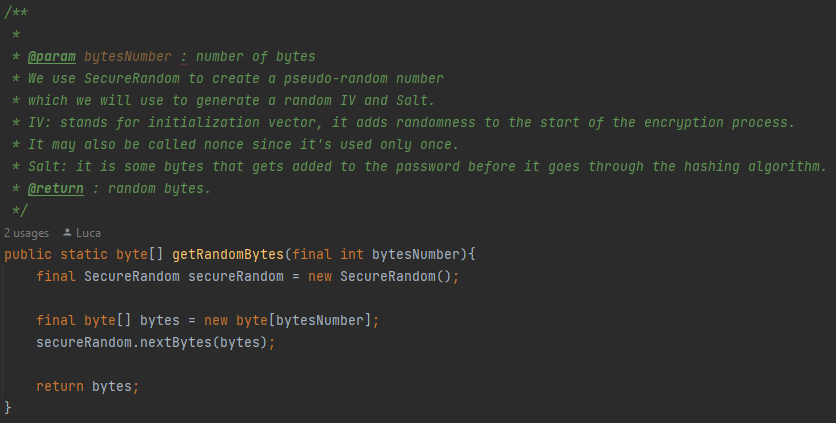
\includegraphics[width=1\textwidth, height=1\textheight, keepaspectratio]{./images/code/java/nonce_getRandomBytes.PNG}
	\caption{Nonce}
	\label{fig:nonce_getRandomBytes}
\end{figure}

\textsf{\small Col metodo \emph{getKeyFromPassword} otteniamo la chiave dalla password assieme alla salatura.} %TODO: 

\begin{figure}[H]
	\centering
	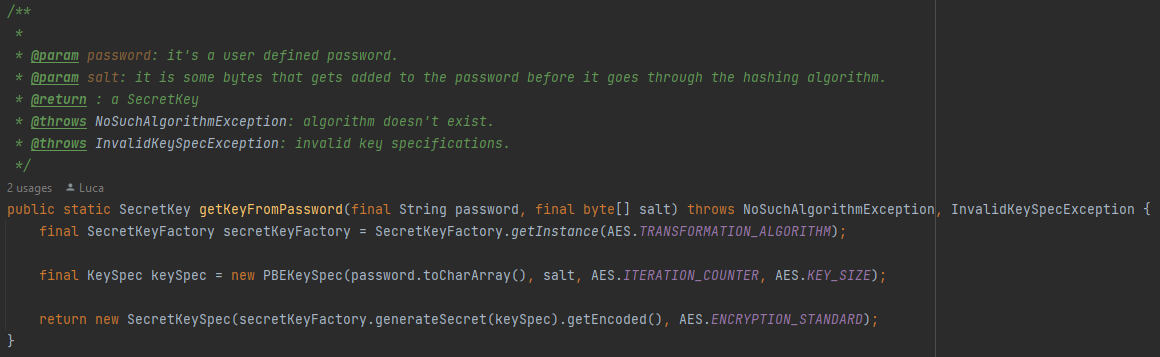
\includegraphics[width=1\textwidth, height=1\textheight, keepaspectratio]{./images/code/java/getKeyFromPassword.PNG}
	\caption{Password}
	\label{fig:getKeyFromPassword}
\end{figure}

\textsf{\small Nel metodo \emph{encrypt()} otteniamo la salatura e l'IV attraverso il metodo \emph{getRandomBytes()} e la chiave attraverso \emph{getKeyFromPassword()}. Dopodiché, inizializziamo il cifrario, cifriamo il messaggio e restituiamo il messaggio cifrato, assieme alla salatura e all'IV.} %TODO: 

\begin{figure}[H]
	\centering
	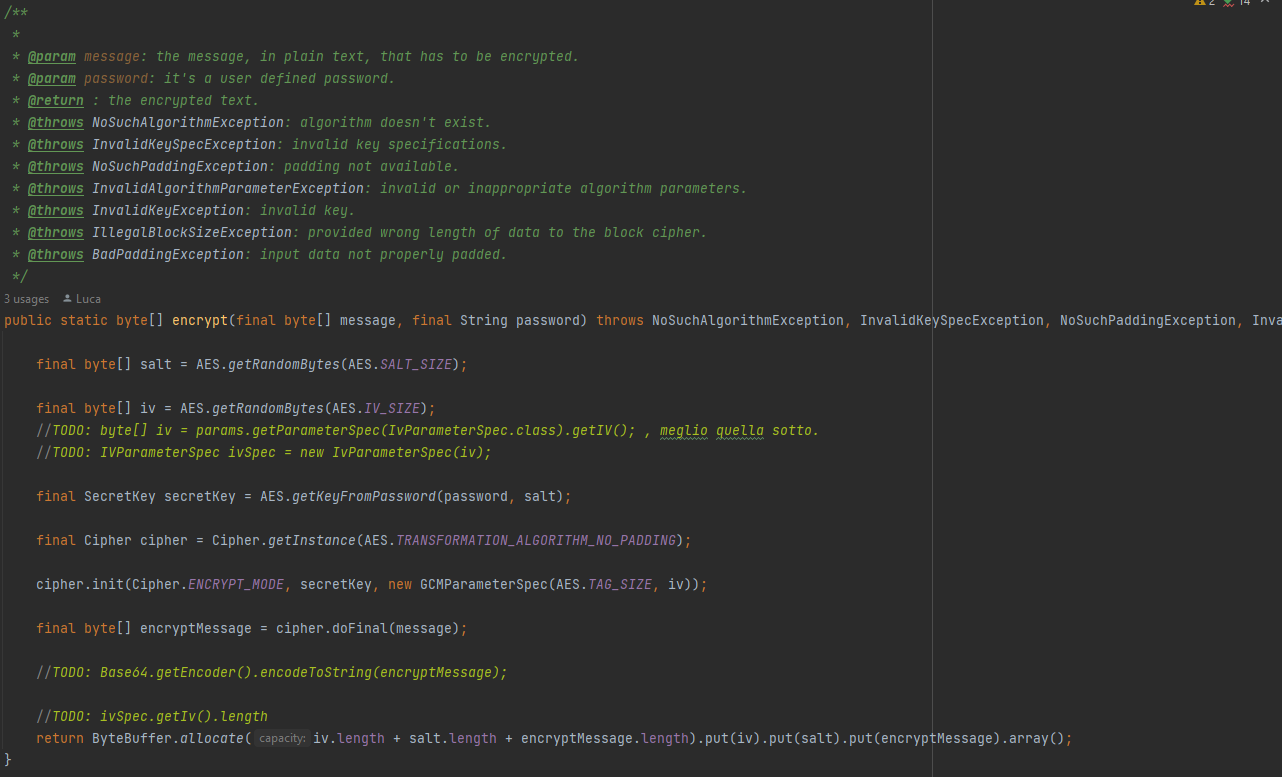
\includegraphics[width=1\textwidth, height=1\textheight, keepaspectratio]{./images/code/java/encrypt.PNG}
	\caption{Cifratura}
	\label{fig:encrypt_java}
\end{figure}

\textsf{\small Nel metodo \emph{decrypt()} otteniamo l'IV e il sale dal messaggio e recuperiamo la password, dopodiché inizializziamo il cifrario e decifriamo il messaggio.} %TODO: 

\begin{figure}[H]
	\centering
	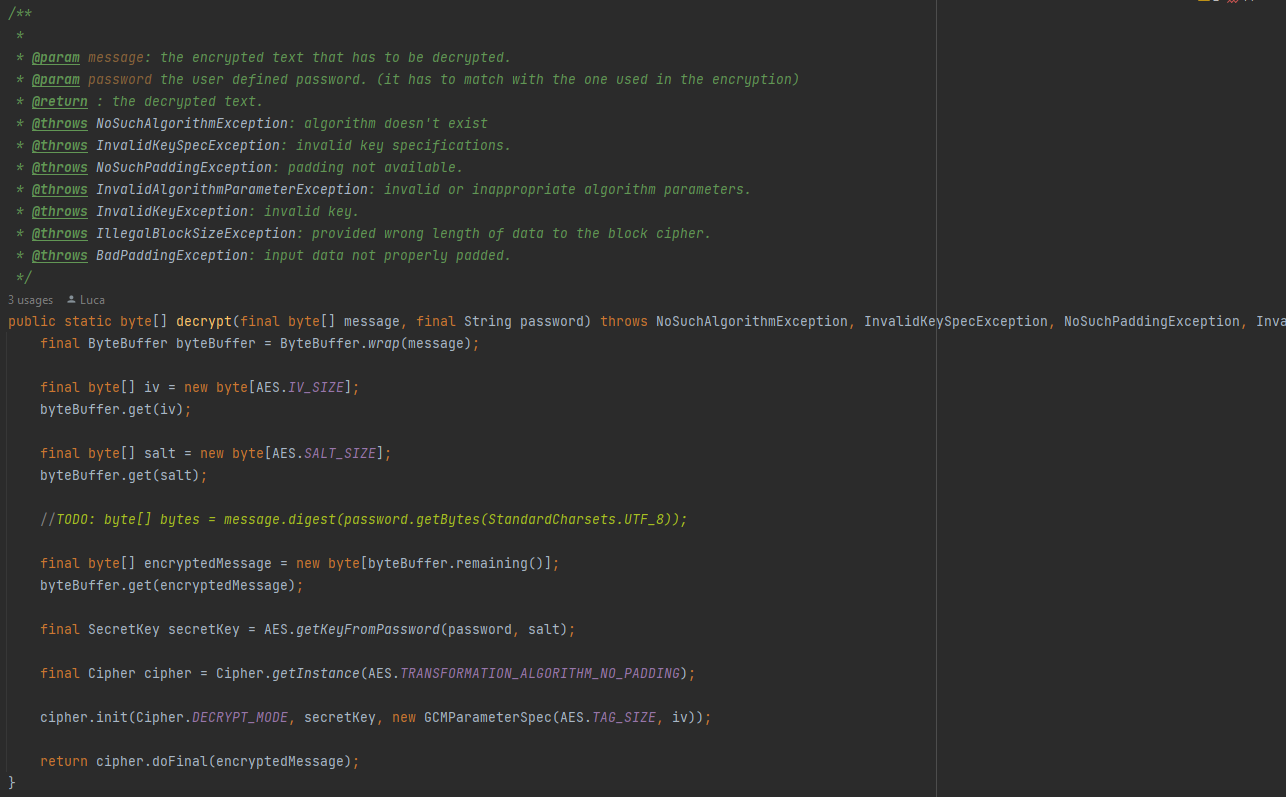
\includegraphics[width=1\textwidth, height=1\textheight, keepaspectratio]{./images/code/java/decrypt.PNG}
	\caption{Decifratura}
	\label{fig:decrypt_java}
\end{figure}

\textsf{\small In \emph{encryptFile} ci avvaliamo del metodo \emph{encrypt} per cifrare. Leggiamo i dati presenti nel file \emph{inputFilePath} e scriviamo il testo cifrato nel file \emph{outputFilePath}.} %TODO: 

\begin{figure}[H]
	\centering
	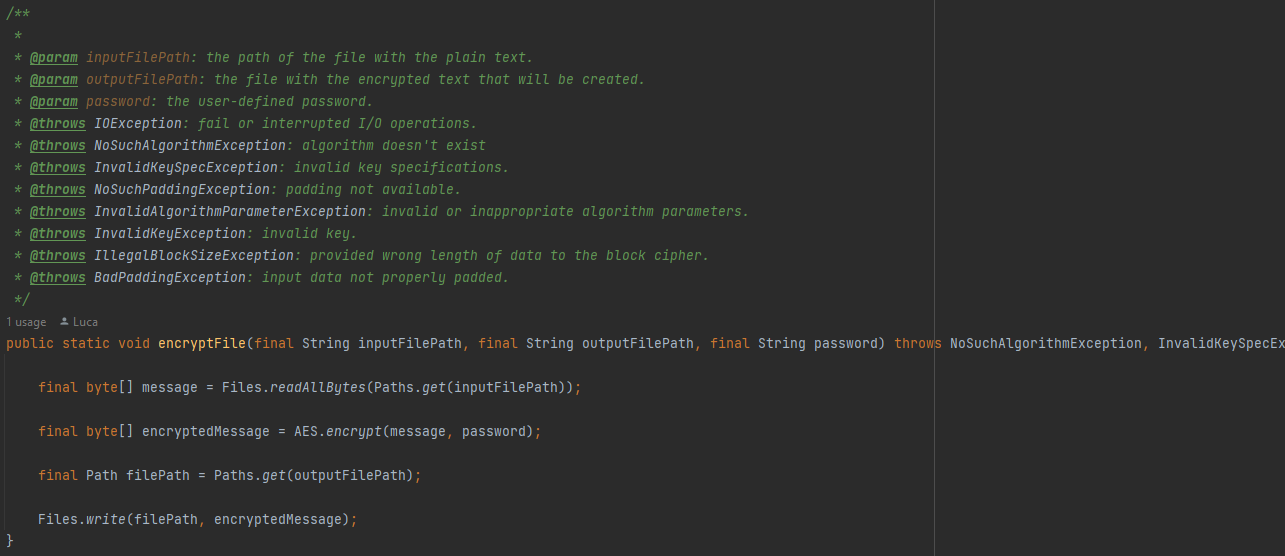
\includegraphics[width=1\textwidth, height=1\textheight, keepaspectratio]{./images/code/java/encryptFile.PNG}
	\caption{Funziona per la cifratura di un File}
	\label{fig:encryptFile}
\end{figure}

\textsf{\small Per \emph{decryptFile} adoperiamo il metodo \emph{decrypt} per decifrare il messaggio cifrato presente nella path indicata dalla variabile \emph{encryptedFilePath}.} %TODO: 

\begin{figure}[H]
	\centering
	\includegraphics[width=1\textwidth, height=1\textheight, keepaspectratio]{./images/code/java/decryptFile.PNG}
	\caption{Funziona per la decifrazione di un File}
	\label{fig:decryptFile}
\end{figure}

%\textsf{\small } %TODO: 

% -------------------------------- FINE CAPITOLO ----------------------------------------
	
	\include{Le_modalità_di_AES}
	
	%TODO: Prima dell'implementazione facciamo: "Le modalità di AES" oppure anche prima del capitolo "La matematica dietro AES" oppure anche no!
	
	%TODO: Implementazione %TODO: oppure dipende dall'implementazione, se nell'implementazione c'è solo AES, allora la parte delle Modalità la metto dopo, altrimenti prima.
	
	%TODO: Pros e Cons (Tipi Attacchi su AES, vulnerabilità?, ecc.) %TODO: volendo resistance to linear and differential cryptoanalysis, wide tail strategy, impractical related key attacks.
	
	%TODO: Conclusioni
	
	%TODO: Bibliografia e Indice Analitico.
	
	\backmatter
	
\end{document}

% ----------------------------- END DOCUMENT -----------------------------------------